
\documentclass[ngerman]{scrreprt}  


\usepackage{babel}


\author{Ziad Bougrine}

\usepackage{url}
\usepackage{titling}
\usepackage{graphicx}
\graphicspath{ {./pictures/} }
\usepackage{xcolor}
\usepackage{eso-pic,lipsum}
\usepackage{biblatex}
\usepackage{lmodern}
\usepackage{algorithm}
\usepackage{algpseudocode}
\usepackage{tabularx}
\usepackage{tikz}


\begin{document}
	\begin{titlepage}
		%----------------------------------------------------------------------------------------
		%	LOGO SECTION
		%----------------------------------------------------------------------------------------
		\begin{tikzpicture}[remember picture , overlay]
			\node [xshift=1cm, yshift=-5cm](a) at (current page.north west){
				
\includegraphics{fh_logo_links}};
		\end{tikzpicture}
		
		\newcommand{\HRule}{\rule{\linewidth}{0.5mm}} 
		
		\center 
		
		%----------------------------------------------------------------------------------------
		%	HEADING SECTIONS
		%----------------------------------------------------------------------------------------
		
		\textsc{\LARGE University of Applied Sciences}\\[1.5cm] 
		\textsc{\Large Seminararbeit}\\[0.5cm] 
		\textsc{FACHBEREICH09} \\
		\textsc{Angewandte Mathematik und Informatik}\\
		\vspace{4cm}
		
		%----------------------------------------------------------------------------------------
		%	TITLE SECTION
		%----------------------------------------------------------------------------------------
		
		\HRule \\[0.4cm]
		{ \huge \bfseries Blockchain- Technologie : \texttt{Analyse von Proof of Work (Bitcoin)}}\\[0.4cm] % Title of your document
		\HRule \\[1.5cm]
		
		%----------------------------------------------------------------------------------------
		%	AUTHOR SECTION
		%----------------------------------------------------------------------------------------
		
		\begin{minipage}{0.4\textwidth}
			\begin{flushleft} \large
				\emph{Author:}\\
				Ziad \textsc{Bougrine} \textit{(3560356)} \\
			\end{flushleft}
		\end{minipage}
		~
		\begin{minipage}{0.4\textwidth}
			\begin{flushright} \large
				\emph{Lecturer:} \\
				prof. dr. Volker \textsc{Sander} \\
				prof. dr. Walk \textsc{Lukas} \\
			\end{flushright}
		\end{minipage}\\[2cm]
		
		{\large \today}\\[2cm]
		
		\vfill 
		
	\end{titlepage}
	
	\newpage
	Diese Arbeit ist von mir selbständig angefertigt und verfasst. Es sind keine anderen als die angegebenen Quellen und Hilfsmittel benutzt worden. \\ \\
	Ziad Bougrine ........................................... \\
	\vspace{16cm}
	
	\begin{normalsize}
		Diese Arbeit wurde betreut von:
	\end{normalsize}
	\begin{enumerate}
		\item Prüfer : \textbf{Volker, Sander}
		\item Prüfer : \textbf{Walk, Lukas}
	\end{enumerate}	



  \begin{abstract}
  	\begin{center}
  		 \begin{LARGE}
  		\textbf{Zusammenfassung auf Deutsch }
  		\end{LARGE}
  	\end{center} 
    Dieser Bericht ist eine Seminararbeit für mein 5. Semester, ich möchte mich wirklich bei den Professoren bedanken, dass sie mir diese Arbeit gegeben haben. Es war wirklich mein erster Schritt, um mit der Blockchain-Entwicklung zu beginnen, in dem ich viele Informationen über Kryptowährungen und Blockchain-Netzwerke recherchiert habe, außerdem habe ich die Funktionsweise von Kryptowährungen basierend auf Proof-Of-Work verstanden. Dieser Bericht enthält eine Zusammenfassung aller Informationen über Blockchain, in technischer und theoretischer Hinsicht. Er beinhaltet auch die Investitionsmethode und das Gewinnen von Geld aus Bitcoin und anderen Kryptowährungen auf Basis von Proof-Of-Work.
  \end{abstract}

	\begin{abstract}
   	\begin{LARGE}
   	\begin{center}
   		\textbf{Abstract in Englisch}
   	\end{center}
	\end{LARGE}
   	This report is a seminar work for my 5th semester, I really want to thank the professors for giving me this work. It was really my first step to start with blockchain development, in which I researched a lot of information about cryptocurrencies and blockchain networks, also I understood the working of cryptocurrencies based on Proof-Of-Work. This report contains a summary of all the information about Blockchain, in technical and theoretical aspects. It also includes the investment method and making money from Bitcoin and other cryptocurrencies based on Proof-Of-Work.

   \end{abstract}

  \tableofcontents


\chapter{Einleitung}
Blockchain ist seit den späten 2000er Jahren eine der wichtigsten Technologien im Bereich digitaler Transaktionen. Im Jahr 2008 veröffentlichte eine Person oder Gruppe von Personen unter dem Namen Satoshi Nakamoto ein Whitepaper mit dem Titel "Bitcoin: A Peer-to-Peer Electronic Cash System". Vier Monate später, am 3. Januar 2009, wurde der Genesis-Block erstellt, der den Beginn und Tag 0 des Bitcoin- und Blockchain-Netzwerks markierte. Die Blockchain wurde entwickelt, um als öffentliches Hauptbuch für Bitcoin-Transaktionen zu dienen und basiert auf der "Proof-of-Work"-Methode, um die Schaffung und den Handel von Bitcoin und anderen Kryptowährungen während der Finanzkrise 2007/08 zu unterstützen. Heutzutage gibt es viele Kryptowährungen wie Litecoin (2011), Ethereum (2015) und Dogecoin (2013).\\ \\
Die Implementierung der Blockchain in Bitcoin machte es zur ersten digitalen Währung, die das Problem der doppelten Ausgaben ohne die Notwendigkeit einer vertrauenswürdigen zentralen Behörde löst. Einer der Hauptvorteile von Blockchain ist, dass jeder erstellte Block, der einen Datensatz enthält, unveränderlich ist und seine Authentizität von der gesamten Gemeinschaft autorisierter Benutzer und nicht von einer einzigen zentralen Behörde überprüft werden kann. Das System ist daher darauf ausgelegt, die Transparenz und Rechenschaftspflicht von digitalisierten Transaktionen zu verbessern.\\ \\
Ein Beispiel: Stellen Sie sich ein Transaktionsbanksystem vor, das von einem Server oder Systemadministrator verwaltet wird. Dies könnte die Wartung des Systems, das Verwalten, Löschen und Hinzufügen von Benutzer- oder Transaktionsinformationen zur Datenbank umfassen. Es könnte auch bedeuten, dass der Administrator behauptet, dass Sie ihm 10.000 € schulden, was gefährlich ist.
Das ist der Grund, warum die Blockchain-Technologie erfunden wurde. Indem es immer für alle sichtbar im Hauptbuch aufgezeichnet wird, wenn Geld von einem Konto auf ein anderes überwiesen wird, kann jeder Benutzer die Transaktion überprüfen und sicherstellen, dass sie korrekt ist.\\ \\



\chapter{Einführung in die Blockchain}

%##############################
%#           Section 1        #
%##############################
\section{Blockchain Definition}
Die \textbf{Blockchain} ist eine ständig wachsende Liste von Datensätzen, die in einzelnen Blöcken organisiert sind. Sie dient als öffentliches Hauptbuch, in dem Personen Datensätze einsehen und erstellen können. Jeder Block besteht aus Daten, einem Hash, dem Hash des vorherigen Blocks und einem Zeitstempel. Das Wesentliche an der Blockchain ist, dass wir spätere Transaktionen auf früheren Transaktionen aufbauen und deren Richtigkeit bestätigen können, indem wir die Kenntnis der früheren Transaktionen nachweisen. Auf diese Weise wird es unmöglich gemacht, die Existenz oder den Inhalt früherer und späterer Transaktionen zu manipulieren. Andere Teilnehmer der dezentralen Buchhaltung erkennen eine Manipulation der Blockchain an der Inkonsistenz der Blöcke..\\
\\
\\
\\
Die \textbf{Blockchain} ist ein verteiltes Hauptbuch, das sich selbst reguliert, das heißt, dass es keine Person gibt, die Kontrolle oder Veränderungen vornehmen kann. Stattdessen tragen Tausende von Benutzern, die am Blockchain-Netzwerk teilnehmen, dazu bei, es funktionsfähig zu halten. Wenn eine Person versucht, das System zu betrügen, wird sie schnell als Betrugserkennung markiert, da das gesamte Netzwerk sie überprüft.


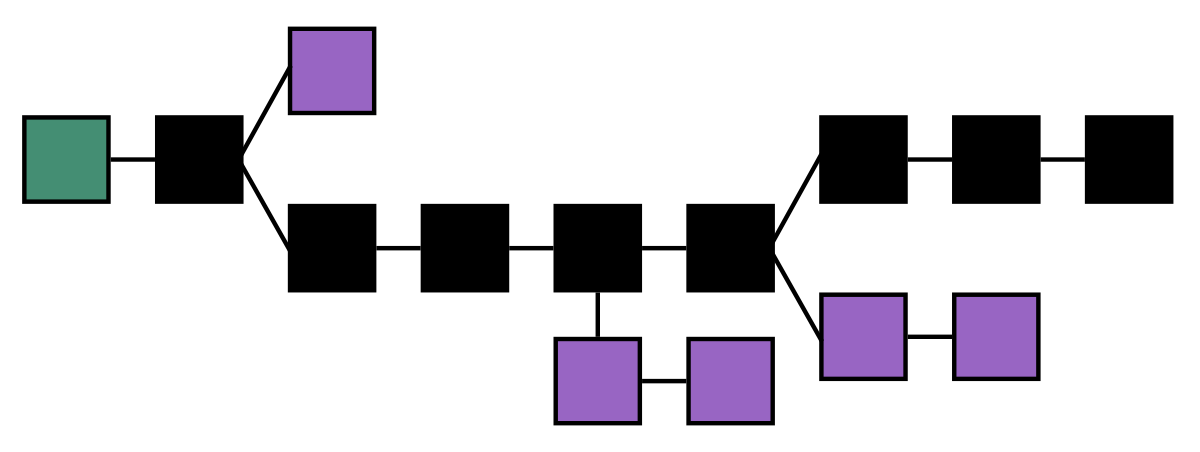
\includegraphics[width=\linewidth]{1.png}

\section{Konstruktion des Blocks}
Ein Block speichert Informationen über Transaktionen, Zeitstempel, vorherigen Hash, Block-Hash.
\begin{itemize}
\item \textbf{Magische Zahl :} Nummer, die diesen Block als Teil des Netzwerks einer bestimmten Kryptowährung identifiziert.
\item \textbf{Transaktionen :} die Hauptinformationen und auch den größten Teil des Blocks
\item \textbf{Transaktionszähler :} die Anzahl der im Block gespeicherten Transaktionen
\item \textbf{Block Größe :} die maximale Größe der Informationen, die der Block enthält
\end{itemize} 
Ein Block enthält viele Informationen, belegt jedoch nicht viel Speicherplatz. Nehmen wir diese Elemente als Beispiel:
Was ist die Hauptinformationen, die ein Block (Transaktionen) enthält?
\begin{itemize}
\item \textbf{Version:} Sie ist benutzbar, um einen neuen Block zu erstellen und um eine neue Version von Software zu identifizieren. Es ist auf 4 Bytes (4 x 8 „bits“) codiert.
\item \textbf{Vorheriger Block-Hash:} Enthält einen Hash des Headers des vorherigen Blocks (md5, sha256 ...). Es ist auf 32 Bytes (32 x 8 = 256 „bits“) codiert.
\item \textbf{Hash Merkle root:} Hash of transactions in the Merkle tree of the current block. Es ist auf 32 Bytes (32 x 8 = 256 „bits“) codiert.
\item \textbf{Time:} Erstellungszeit des Blocks. Es ist auf 32 Bytes (32 x 8 „bits“) codiert.
\item \textbf{Bits:} Es ist ein Wert, der die Schwierigkeitsbewertung des Ziel-Hashes und die Schwierigkeit beim Lösen der „Nonce“ angibt. Es ist auf 32 Bytes (32 x 8 „bits“) codiert.
\item \textbf{Nonce:} Es ist die magische Zahl, die der Miner lösen muss, um einen Block im Blockchain-Netzwerk zu verifizieren und zu schließen.\\ \\ \\ \\ \\
\end{itemize}

\color{green}
\Large{\textbf{Information :}} 
\color{black}
\normalsize
Die Miner setzen ihre Rechenleistung ein, um mithilfe von Zufallszahlen (Bruteforce) die Nonce im Hash zu erraten. Sobald die Nonce erfolgreich bestimmt wurde, wird der Hash verifiziert und der Block geschlossen. Anschließend wird ein neuer Block mit einem Header erstellt und der Prozess wiederholt sich. Die Nonce ist von Interesse für Miner, da sie einen wichtigen Bestandteil des Mining-Prozesses darstellt, bei dem versucht wird, den Hash zu lösen. \\ \\ \\

\large
\underline{\textbf{Was sind Merkle-Bäume?}} \\ \\
\normalsize
Es handelt sich um eine Datenstruktur in Form eines Binärbaums, die in Bitcoin und Kryptowährung weit verbreitet ist und zur effizienten und sicheren Kodierung von Daten verwendet wird.




\section{Blockchaining-Mechanismus}
\textbf{Die Funktionsweise der Blockchain} ähnelt der einer verketteten Liste, da sie aus einer Reihe von Blöcken besteht, die jeweils durch einen Hash des aktuellen Blocks und einen Hash des vorherigen Blocks verbunden sind. Dieser Mechanismus ermöglicht es, über die Kette zu iterieren, ähnlich wie bei einer verketteten Liste, in der jeder Knoten einen Zeiger auf den vorherigen Knoten enthält.

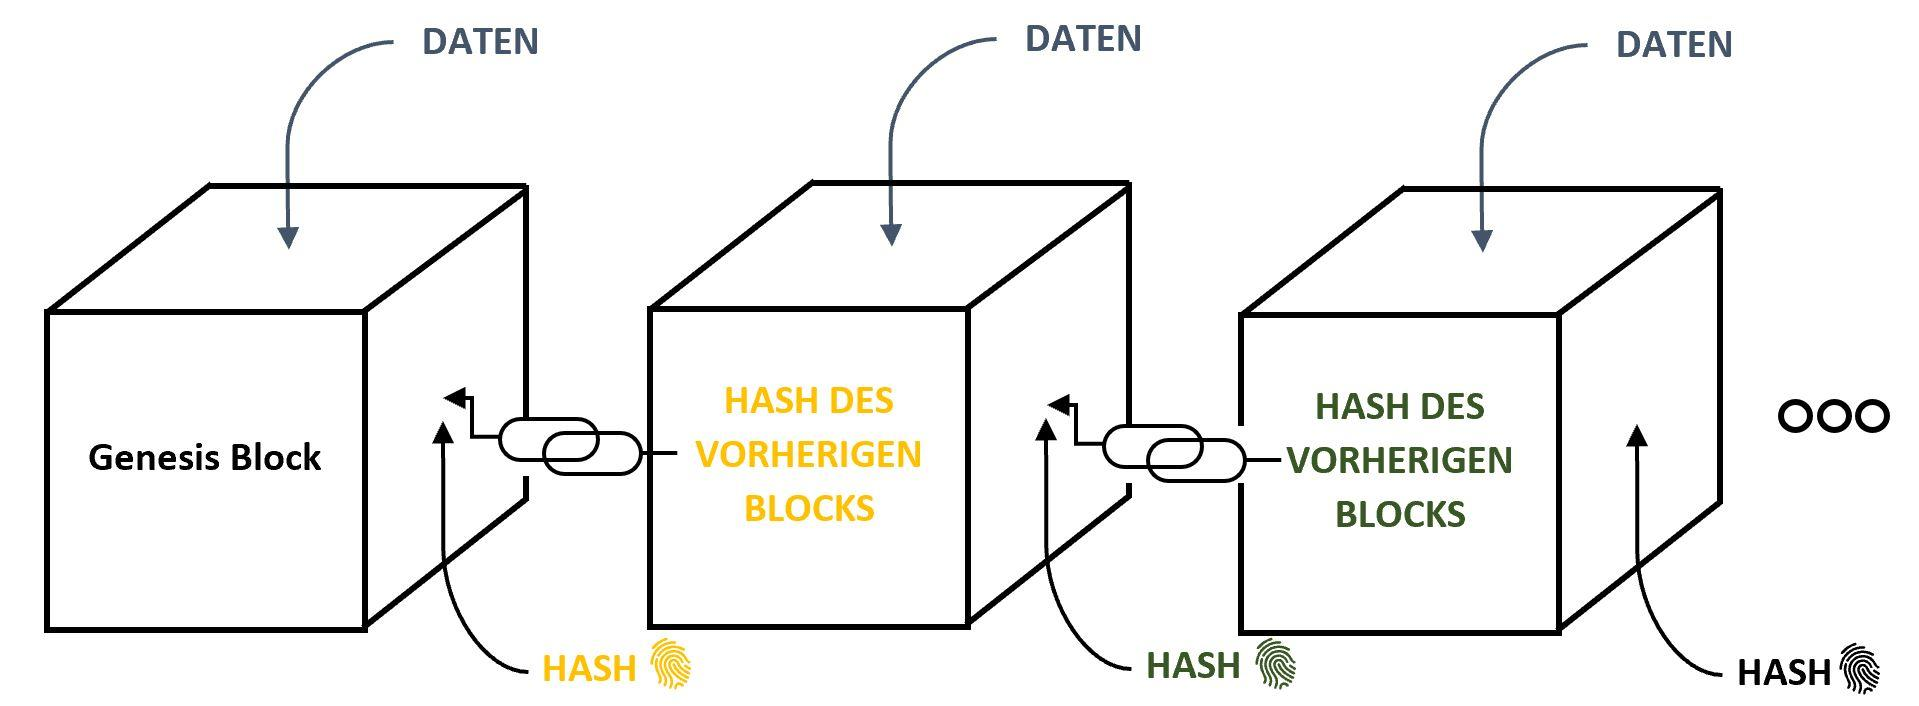
\includegraphics[width=\linewidth]{2}


\textbf{Der erste Block der Kette wird als Genius-Block bezeichnet.} \\ \\ \\


In solchen Fällen sollte man immer bedenken, welche Handlungen von verdächtigen Personen ausgehen könnten, beispielsweise das Modifizieren oder Manipulieren der Daten im Block (i). Dies führt zu einer Änderung des tatsächlichen Blocks i und macht den vorherigen Hash im Block (i+1) ungültig. Dies bedeutet, dass das Ändern eines Blocks alle darauf folgenden Blöcke in der Blockchain ungültig macht, was die Integrität der Kette beweist.\\ \\ \\ 
\color{red}
\Large{\textbf{Achtung :}}
\color{black}
\textbf{Ist dieser Mechanismus gesichert?}\\ \\
\normalsize
 	
Der Einsatz von Hashes allein reicht nicht aus, um Manipulationen zu verhindern. Da Computer heutzutage sehr schnell sind und Tausende von Hashes berechnen können, besteht technisch gesehen die Möglichkeit, einen Block zu manipulieren und alle nachfolgenden Hashes der nachfolgenden Blöcke erneut zu berechnen, um das Blockchain-Netzwerk wieder gültig zu machen. Aus diesem Grund verwendet die Blockchain den sogenannten "Proof of Work (POW)", um dieses Problem zu vermeiden.	



\chapter[Theoretische Seite der Proof-Of-Work-Methode]{Einführung in die „Proof-Of-Work“-Methode}	

\section{Was ist Proof-Of-Work ?}
Proof-Of-Work (POW) wurde entwickelt, um zu verhindern, dass Nutzer Blocks in der Blockchain leicht manipulieren. Es verlangt von Minern, eine signifikante Menge an Mühe aufzuwenden, um einen Block zu erstellen. Diese Methode basiert auf verschiedenen Grundprinzipien in der Kryptowährung, wie folgt:

\begin{itemize}
	\item{Der Proof-of-Work-Mechanismus sorgt dafür, dass das Hinzufügen von Blöcken zur Blockchain-Kette mit einer gewissen Schwierigkeit verbunden ist, indem es Miner dazu zwingt, einen gültigen Hash zu finden. Diese Methode wurde so konzipiert, dass etwa alle zehn Minuten ein neuer Block mit einer festgelegten Menge an BTC in die Kette aufgenommen wird. Dies gewährleistet das algorithmische Wachstum der Geldmenge.}
	\item{Die Verwendung von Proof-of-Work ermöglicht es den Nodes, die Integrität der Blockchain zu überprüfen, indem sie diejenige wählen, die den größten Aufwand in Form von Rechenleistung darstellt. Auf diese Weise ist es einfach zu erkennen, welche Blockchain die authentische ist.}
	\item{Die Verwendung von Proof of Work dient dazu, das Blockchain-Netzwerk vor Angreifern zu schützen, da diese eine größere Energiemenge in das Netzwerk einspeisen müssten als alle anderen verfügbaren Miner insgesamt über einen längeren Zeitraum. Dies ist beim Bitcoin aufgrund der enormen Rechenleistung, die benötigt wird, um einen gültigen Block zu erstellen, praktisch unmöglich.}
	\item{Proof of Work ist eine bewährte Methode zur Sicherung von Blockchains und zur Neuverteilung von digitalen Währungen. Im Gegensatz zu Fiatgeld, das von Zentralbanken gedruckt werden kann, erfordert die Erschaffung von Coins in einem Proof-of-Work-System einen tatsächlichen Einsatz von Ressourcen. Dadurch wird ein fairer Mechanismus für die Verteilung von Coins gewährleistet.}
\end{itemize}

\section{Wie funktioniert Proof of Work bei einer Blockchain ?}
Der Proof-of-Work-Mechanismus erfordert, dass Miner mithilfe von Bruteforce-Methoden versuchen, eine Nonce zu finden, die bestimmte Eigenschaften aufweist, wodurch Milliarden von Berechnungen durchgeführt werden. Sobald ein solches Ergebnis erzielt wurde, wird den Minern eine Belohnung in Form einer Blocksubvention gewährt. Dieser Prozess wird als Mining bezeichnet.\\ \\ \\ \\
\textbf{Diese beschreiben den Prozess einer Transaktion im Blockchain-Netzwerk. \\ }
\begin{itemize}
	\item{Die Blockchain generiert einen Block, der alle Transaktionen enthält, die in einem bestimmten Zeitraum stattgefunden haben.}
	\item{Der Verifizierer wird die Integrität der Transaktionen überprüfen, um sicherzustellen, dass sie legitim sind.}
	\item{Die Miner im Netzwerk überprüfen dann die Legitimität dieser Transaktionen und führen anschließend eine Suche durch, indem sie die Nonce erraten. Der erfolgreiche Miner, der als erstes die Lösung findet, wird mit einer Belohnung und den Transaktionsgebühren belohnt. Dieser Prozess wird als "Mining" bezeichnet. Das Blockchain-Netzwerk wird dann um den Block mit den bestätigten Transaktionen erweitert und wird als Teil der Kette von Blöcken gespeichert.}
	\item{Die Transaktionsbestätigung im Blockchain-Netzwerk wird wiederholt \\}
	
\end{itemize}
\textbf{Dies ist ein sequentielles Diagramm, das erklärt, wie es funktioniert \\}
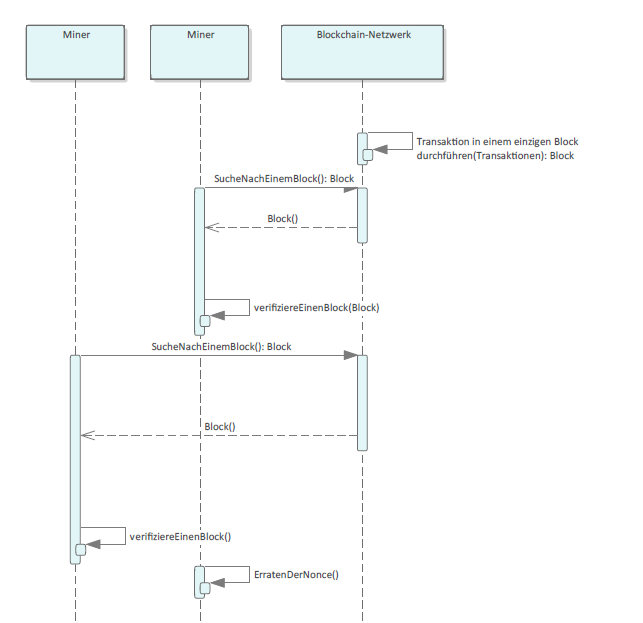
\includegraphics[width=\linewidth]{ProofOfWork1.png} \\ \\
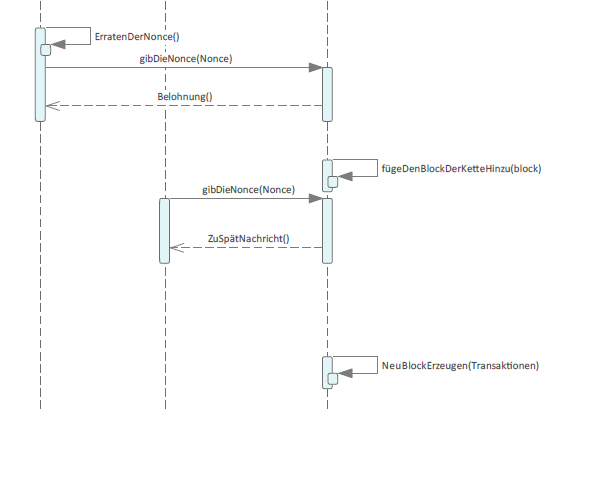
\includegraphics[width=\linewidth]{ProofOfWork2.png}
\section{Wie genau funktionieren die Proof-of-Work-Berechnungen?}
\begin{itemize}
	\item {Die Miner im Blockchain-Netzwerk nutzen Hash-Funktionen, die in ihrer Funktionsweise unumkehrbar sind. Sie können eine beliebig lange Zeichenfolge in eine eindeutige Zeichenfolge festgelegter Länge umwandeln. Die Schwierigkeit besteht darin, ein Ergebnis zu erzielen, das bestimmte Eigenschaften aufweist, die sich aus der Verwendung der Hash-Funktion ergeben. Ein bekanntes Beispiel hierfür ist der Einsatz der SHA-256-Hash-Funktion im Bereich des Minings bei Bitcoin.}
	\item{Die Hash-Funktion ist eine eindeutige, nicht invertierbare mathematische Funktion, die aus einer beliebigen Eingabestring eine feste Länge erzeugt. Sie wird häufig in der Kryptographie und im Blockchain-Bereich verwendet. Im Fall von Kryptowährungen wie Bitcoin wird sie beim Mining verwendet, wobei Miner versuchen, einen Wert mit bestimmten Eigenschaften zu finden, indem sie der Hash-Funktion Zeichenfolgen übergeben. Da die Rückgängigmachung der Hash-Funktion nicht möglich ist, kann der Miner den erhaltenen Wert nicht einfach umkehren und die Eingabe der Hash-Funktion erhalten.}
	\item{Aus diesem Grund gibt es das Konzept \textbf{"Mining"}, Mining ist ein Prozess, bei dem Miner versuchen, die Nonce und die Reihenfolge der Parameter zu erraten, die von einer Hash-Funktion als Eingabe akzeptiert werden, um ein Ergebnis zu liefern. Da es unmöglich ist, die Hash-Funktion umzukehren, um die ursprüngliche Eingabe zu erhalten, müssen Miner eine Vielzahl von Operationen durchführen, um den Wert der Eingabe für die Hash-Funktion zu ermitteln. Dies geschieht durch das Konzept des Minings, bei dem Miner versuchen, die Nonce und die Reihenfolge jedes Parameters, die von der Hash-Funktion als Eingabe akzeptiert werden, zu erraten.}
	\item{Wenn der Block abgebaut wird, überprüfen alle Teilnehmer des Blockchain-Netzwerks die präsentierte Lösung, um zu bestätigen, dass die Gültigkeit der Blockchain aufrechterhalten wird.}
\end{itemize}


\section{Was hat es mit der Schwierigkeit auf sich ?}
\begin{itemize}
\item{Die Schwierigkeit besteht darin, die gewünschte Hash-Ausgabe zu finden. Zum Beispiel Bitcoin, es wird eine Frage gestellt: Wie viele Nullen soll die Ausgabe am Anfang des Strings haben. Je mehr Nullen gefordert sind, desto schwieriger wird es schließlich, den Output zu finden.}
\item{Die Schwierigkeit ist bei Bitcoin immer so gewählt, dass im Schnitt alle zehn Minuten ein neuer Block gefunden werden soll. Dieser Benchmark wird alle zwei Wochen überprüft. Stellt sich heraus, dass in zwei Wochen der Richtwert von 2.016 Blöcken überschritten wurde, also mehr Blöcke als gewünscht gefunden wurden, ist die Schwierigkeit zu gering und wird nach oben korrigiert – und umgekehrt. (check it)}
\end{itemize}

\section{Algorithmus zum Finden einer Nonce}
\begin{itemize}
	\item[--] Es ist von Interesse, die technische Funktionsweise von Proof-of-Work zu untersuchen. Als Erstes betrachten wir eine tatsächliche Blockstruktur von der offiziellen Website "\textit{blockchain.com}".\\
	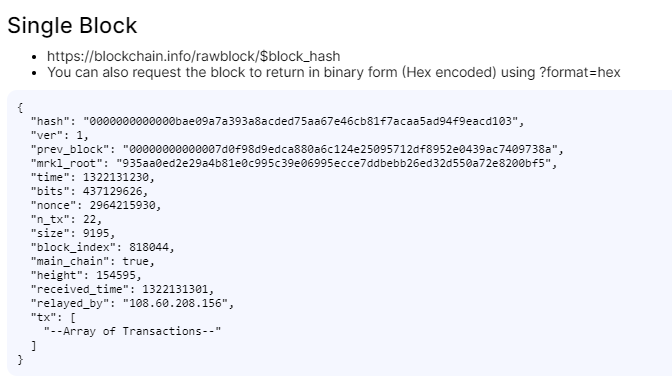
\includegraphics[width=\linewidth]{realblock.png} \\
	\item[--] Und dies ist eine echte Einzeltransaktionsstruktur \\
	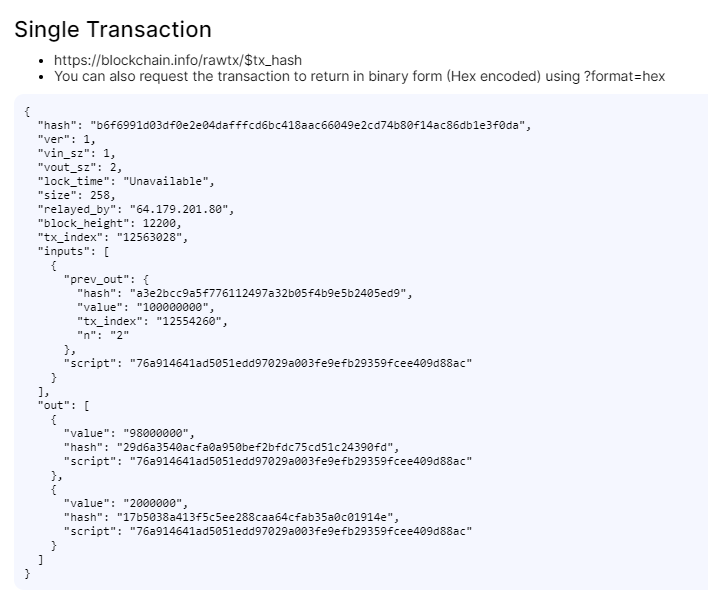
\includegraphics[width=\linewidth]{realtransaction.png} \\ \\
	\item[--] Das nächste Klassendiagramm zeigt die gesamten Daten aus dem realen Blockchain-Netzwerk. Es ist gut, es in Form eines Klassendiagramms zu sehen, um zu erkennen, wie Daten für die Implementierung miteinander in Beziehung stehen \\
	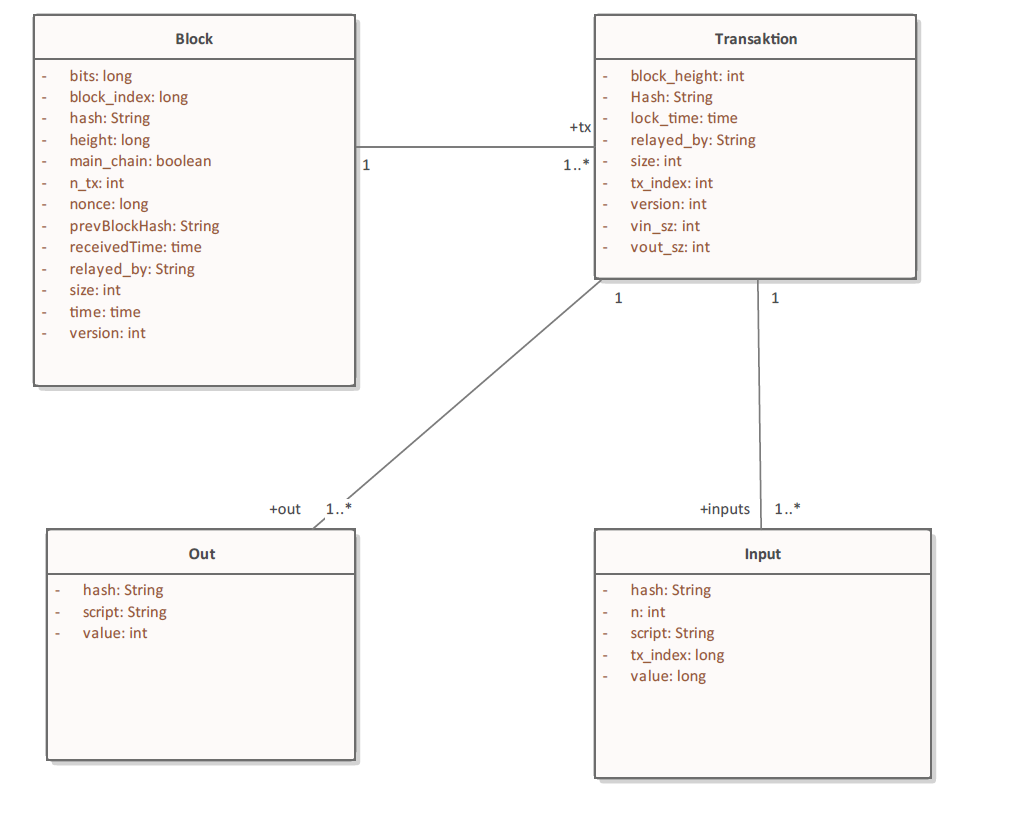
\includegraphics[width=\linewidth]{classOfStructures.png} \\ \\
	\item[--] {Und jetzt erklären wir unseren Algorithmus mit dem Aktivitätsdiagramm, zuerst sollten wir Daten initialisieren, die Initialisierung von Max\textunderscore Nonce \textunderscore Limit, Anzahl der Nullen, für dieses Beispiel werden wir berücksichtigen, dass der Hash mit 4 Nullen beginnen sollte (nur für Informationen, Anzahl von Nullen sind wichtig, es zeigt die Komplexität des Algorithmus, wenn die Zahl hoch ist wie 7 oder 6 Nullen, wird es ein Jahr dauern, die Nonce mit wenig Hardware-Material zu finden.Wir sollten auch unsere i-Inkrement-Variable für die for-Schleife initialisieren } \\ \\
		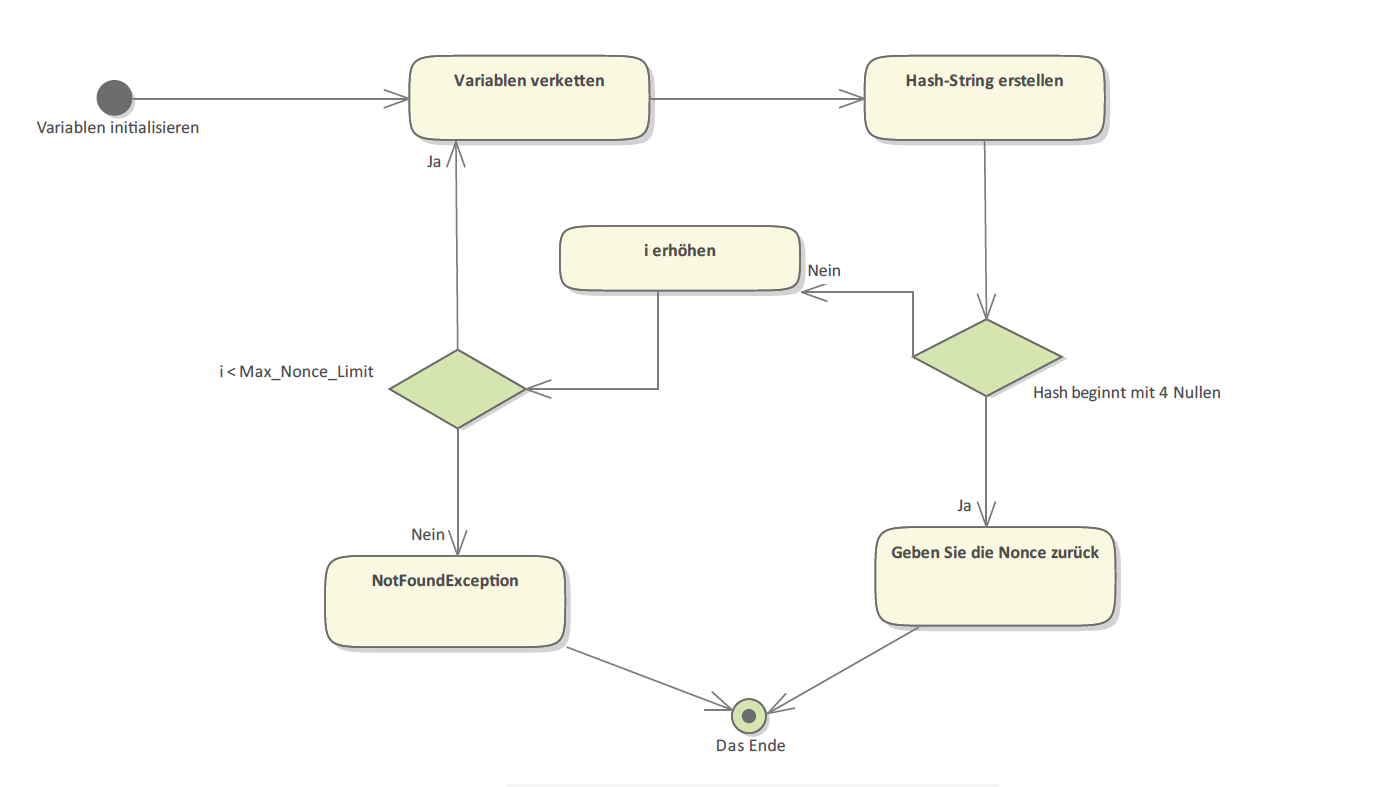
\includegraphics[width=\linewidth]{activity.png} \\ \\
		

	
\end{itemize}
\begin{LARGE}
	\textbf{Dies ist der Algorithmus \textcommabelow der für dieses Beispiel zum Schürfen von Bitcoin geschrieben wurde} \\
\end{LARGE}
\begin{algorithmic}
	\State $i \gets 1$
	\State $MaxNonceLimit \gets 100000000$
	\State $zeros \gets 4$
	\For{$i \ensuremath{<} MaxNonceLimit$}
		\State $data \gets blockNumber + transactions + prvHash + i$
		\State $hashVariable \gets  SHA256(data)$
		\If {$hashVariable.startWith(\textquotesingle 0 \textquotesingle \textasteriskcentered 4)$}
			\Return $i$
		\EndIf
	\EndFor
	
\end{algorithmic}

\section{Sicherheit des Proof-Of-Work}
Was die Sicherheit betrifft, so bietet diese Proof-Of-Work-Methode ein hohes Sicherheitsniveau, da Angreifer über eine größere Energiequelle als andere Blockchain-Knoten verfügen sollten, was im Falle von Bitcoin unmöglich ist.

\newpage
\section{Vor- und Nachteile von Proof-Of-Work}
\textbf{Ich habe diese Tabelle erstellt, um die Vor- und Nachteile dieser Methode genau zu erklären : } \\ \\
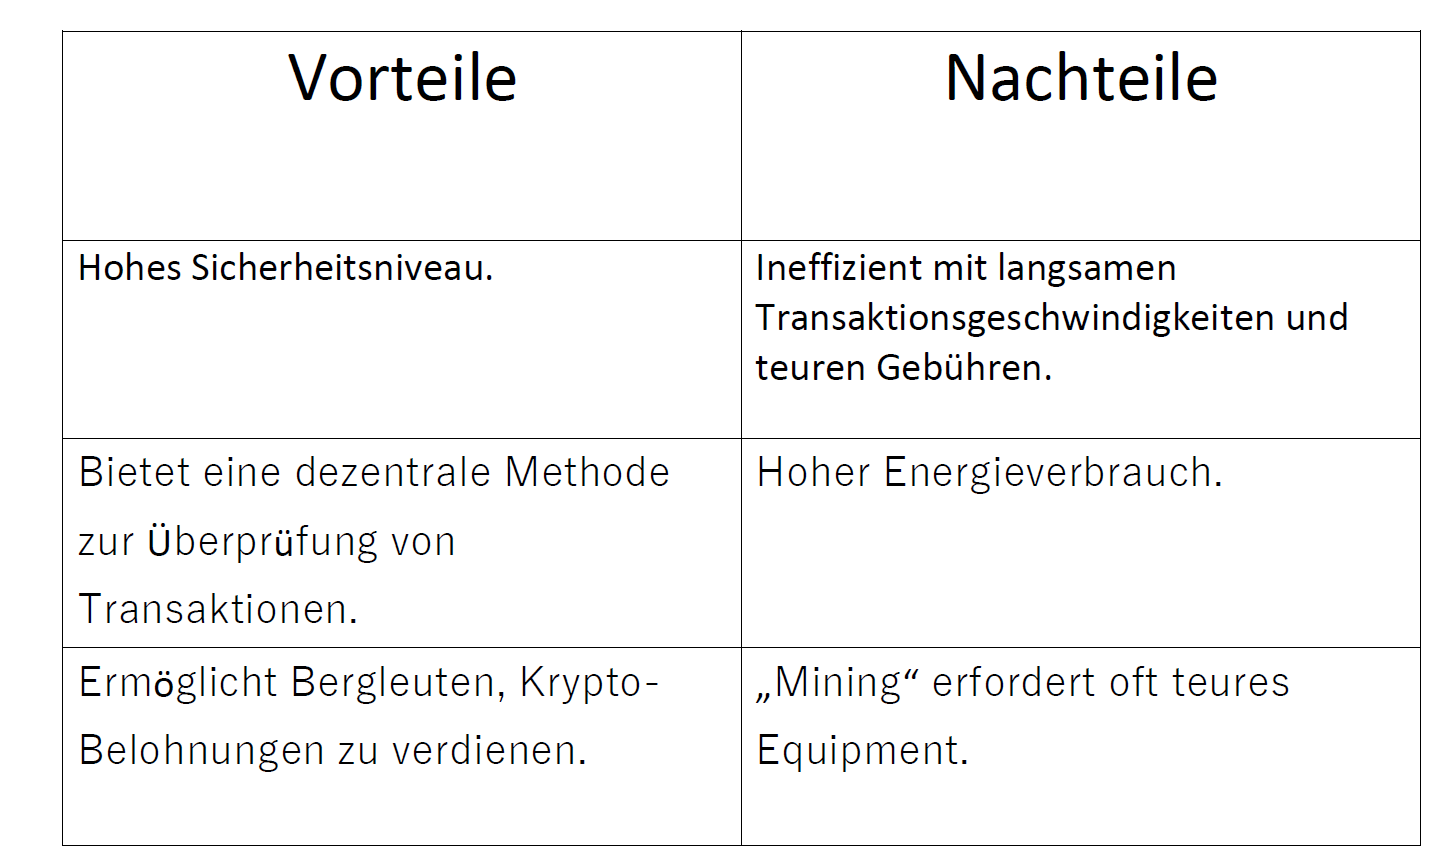
\includegraphics[width=\linewidth]{vornach.png} \\ \\
\textbf{\underline{Eklärung :}}
\begin{itemize}
	\item Für ein hohes Sicherheitsniveau müsste eine spekulative Person, die die Kontrolle über das auf Proof-of-Work basierende Blockchain-Netzwerk übernehmen möchte, 50 \% des
	Blockchain-Netzwerks in Besitz nehmen, was unmöglich ist, und sie benötigt eine Menge Material.
	\item Proof-Of-Work bietet eine dezentralisierte Methode, weil wir keine dritte Partei brauchen, der wir vertrauen, um unsere Transaktionen und Daten zu speichern, was bedeutet, dass alle Transaktionen im öffentlichen Register verfügbar sind und alle Teilnehmer des Blockchain-Netzwerks darauf zugreifen können.
	\item Viele Leute mögen Bitcoin wegen der Mining-Operation, weil alle Miner einige spezielle Hardware "Rig Mining" einrichten können und mit dem Mining von Bitcoin beginnen können und für jede erfolgreiche Mining-Operation eine Belohnung erhalten. \\  \\
\end{itemize}
\textbf{Wo immer es Vorteile gibt, gibt es auch Nachteile. Bei der Proof-Of-Work-Methode gibt es einige Nachteile dieser Methode: }
\begin{itemize}
	\item Transaktionen sind so langsam, weil sie eine Menge von Mining-Operationen benötigen, um einen Block zu überprüfen, der Bitcoin-Transaktionen enthält, auch Blockchain Durchschnitt der Suche nach einem Block nonce ist 1 Nonce pro 10 Minuten, die es so langsam für einen großen Market ist.
	
	\item Um das auf Proof-Of-Work basierende Blockchain-Netzwerk weiterzuführen, ist es eine große Energieverschwendung, weil mindestens 10 Grafikkarten arbeiten und auf extreme Leistung gebracht werden, sie brauchen viel Energie, um rund um die Uhr zu arbeiten, und vergessen Sie nicht die Kühlsysteme, die die Grafikkarten vor hohen Temperaturen schützen. Eine neue Mining-Anlage sollte aber auch erneuerbare Energie erzeugen. Das kostet zwar mehr Material, ist aber mietbar, weil die Mining-Firma keinen externen Strom verbraucht, und der Besitzer kann auch Stromrechnungen sparen. Deshalb können erneuerbare Energien im Bergbau eine gute Rolle spielen. Ich empfehle wirklich die Nutzung von Wind- und Solarenergie, um die benötigte Energie für das Unternehmen bereitzustellen, und das ist auch gut für die Natur, denn man sollte nicht vergessen, dass die externe Energie aus Kernkraftwerken und erneuerbaren Energien stammt. Atomkraft zerstört den Himmel wegen des Gases und stellen Sie sich vor, wenn 30\% der Menschen in Deutschland anfangen würden, Bitcoin ohne erneuerbare Energien zu minen, würden die Energiepreise steigen und auch die Produktion würde steigen. 
	
	\item Das Mining von Bitcoin braucht ein teures Material, weil die Bitcoin-Schwierigkeit heute astronomisch ist, was einige teure Nvidia's Grafikkarten und ein teures Motherboard erfordert, das die Grafik verarbeiten kann, um einen Wettbewerb zu starten. Für meine Meinung auch die teuren Preise, aber es ist rentabel Betrieb, weil Sie das ausgegebene Geld sehr leicht zurück, wenn Sie eine gute Mining-Unternehmen haben. Später werde ich sprechen, wie man eine gute Mining-Unternehmen erstellen kann. \\ \\
	
	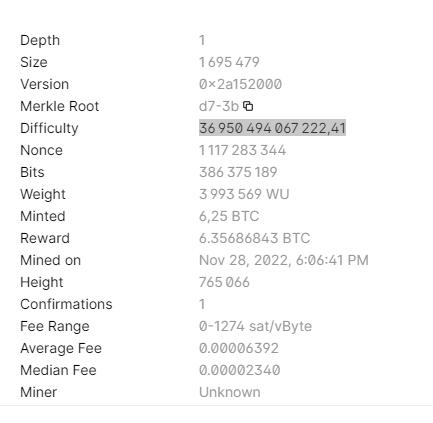
\includegraphics[width=7cm,height=7cm]{difficulty}
\end{itemize}


\chapter{Der Bitcoin-Markt und die Verwendung von Proof of Work}
\section{Münzen}

\begin{itemize}
	\item[--] Bevor ich anfange, mit Ihnen darüber zu sprechen, wie Sie mit Bitcoin Geld verdienen können, möchte ich Ihnen zunächst einige Münzen vorstellen, die die Proof-Of-Work-Methode verwenden
	\begin{itemize}
		\item [--] {Bitcoin Cash} \\ \\ 
		
\includegraphics[width=1.5cm,height=1.5cm]{bitcoincash.png}\\ \\
		
		\item [--] {Bitcoin SV} \\ \\
		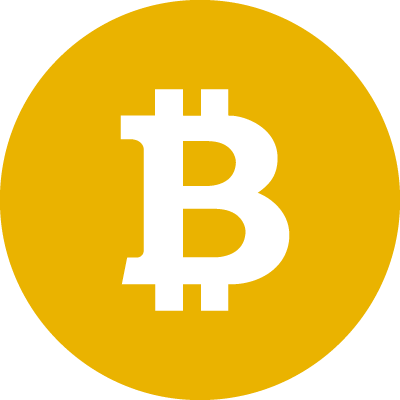
\includegraphics[width=1.5cm,height=1.5cm]{bitcoinsv.png}\\ \\
		\item [--] {Litecoin} \\ \\ 
		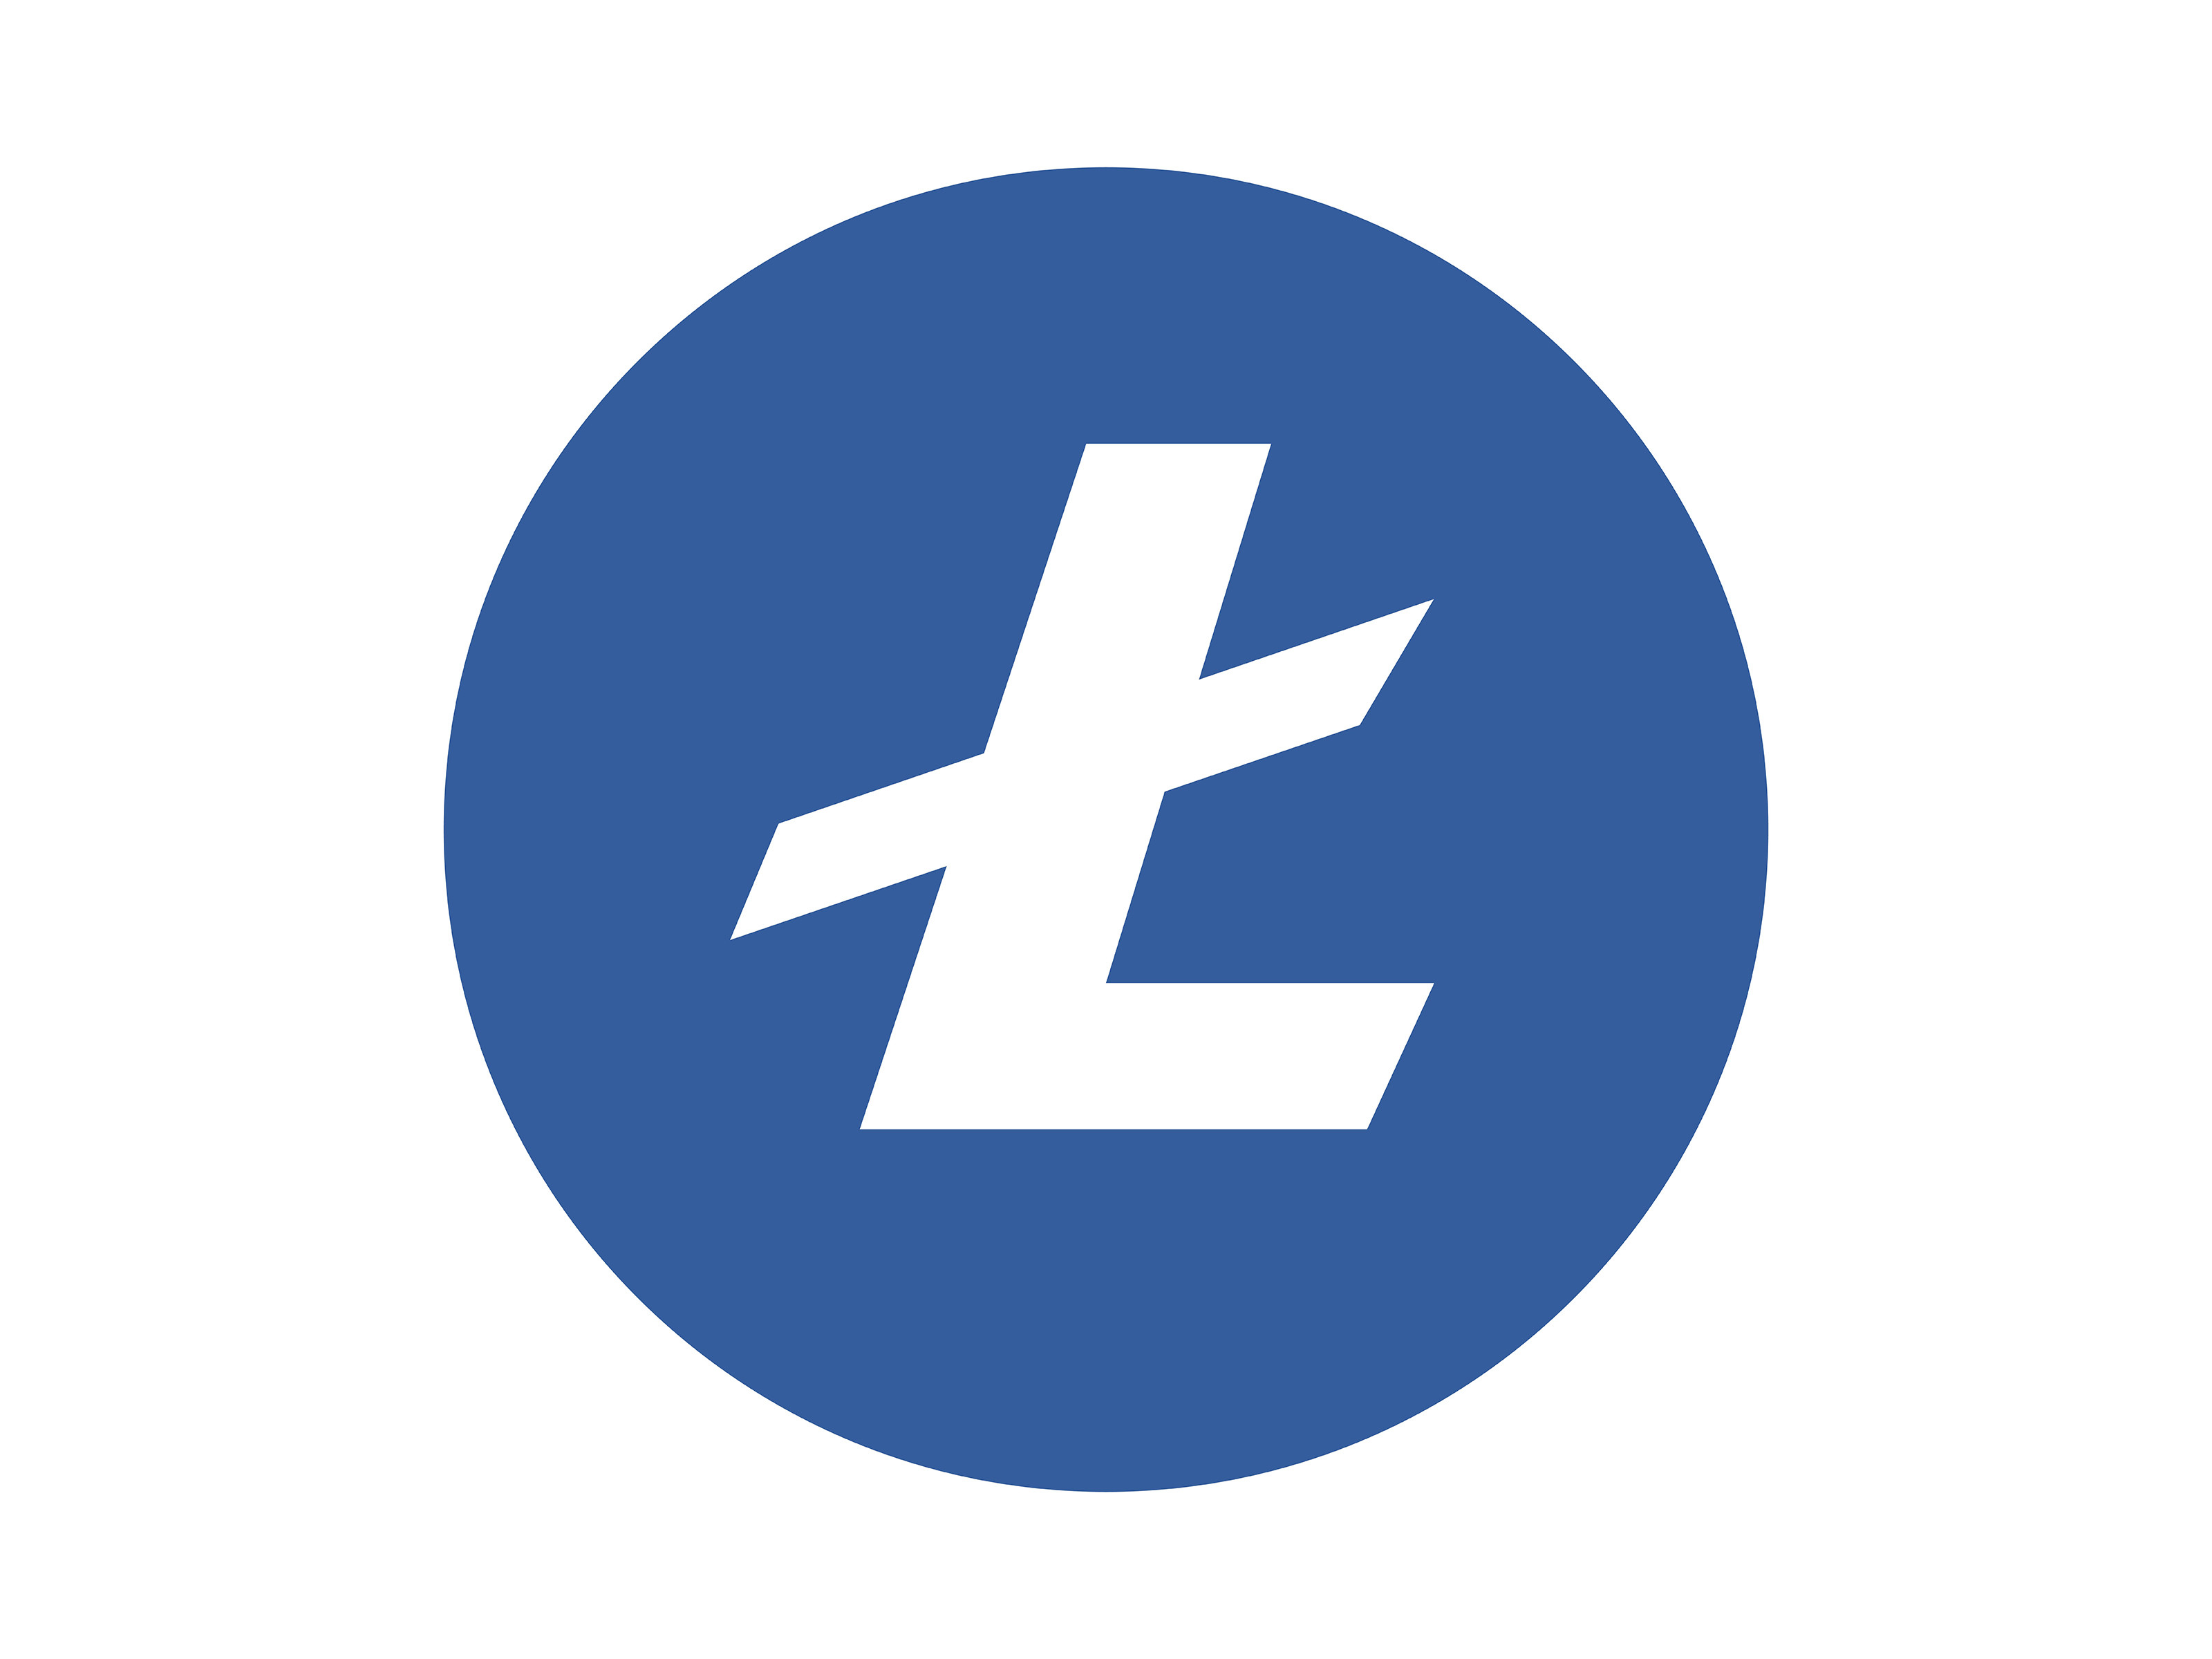
\includegraphics[width=1.5cm,height=1.5cm]{litecoin.jpg} \\ \\
		\item [--] {Dogecoin} \\ \\
		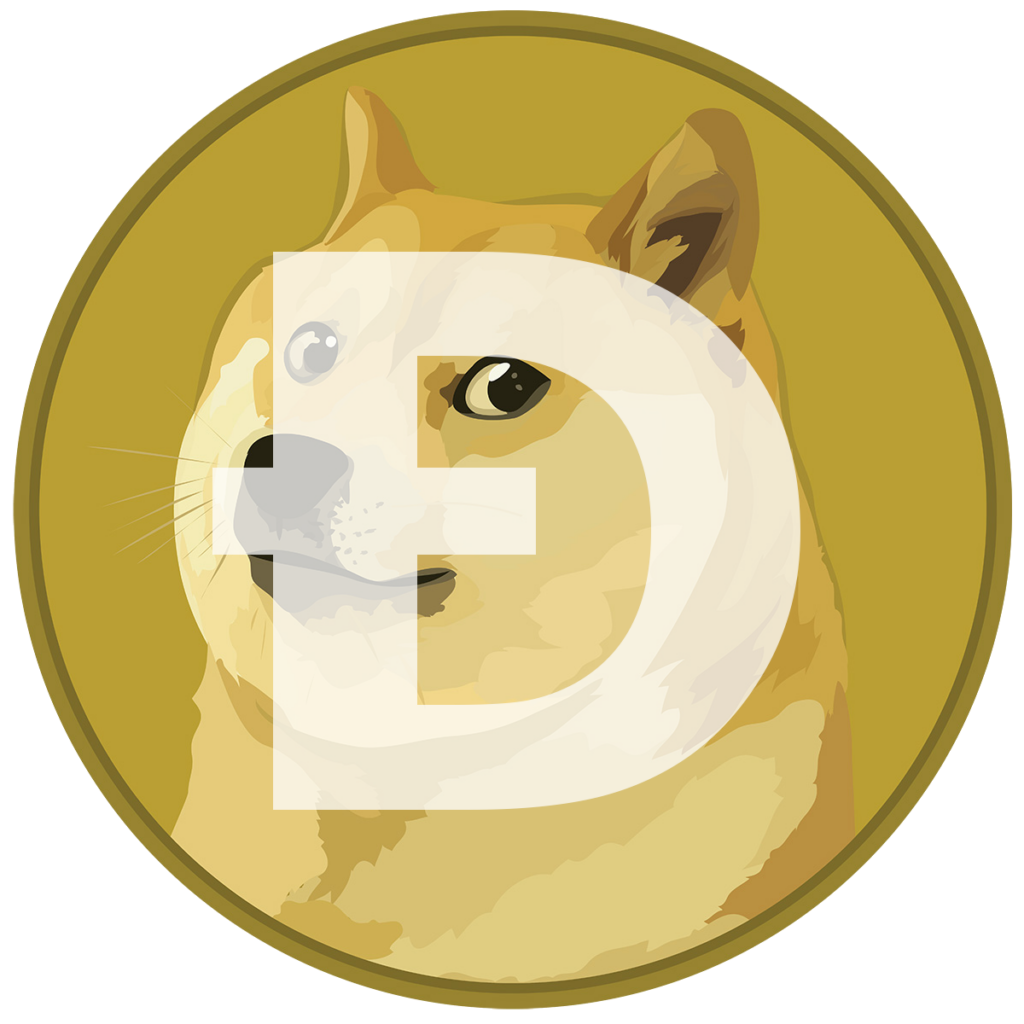
\includegraphics[width=1.5cm,height=1.5cm]{dogecoin.png}\\ \\
		\item [--] {Bitcoin Gold}\\ \\
		
\includegraphics[width=1.5cm,height=1.5cm]{bitcoingold.png}\\ \\



	\end{itemize}
	
	\item[--] Es gibt auch viele andere Kryptowährungen, die nicht auf Bitcoin basieren, aber die Proof-of-Work-Methode verwenden :
	\begin{itemize}
		\item{Ethereum Classic} \\ \\
		
\includegraphics[width=1.5cm,height=1.5cm]{ethereumclassic.png}\\ \\
		\item{Monero}\\ \\
		
\includegraphics[width=1.5cm,height=1.5cm]{monero}\\ \\
		\item{Zcash}\\ \\
		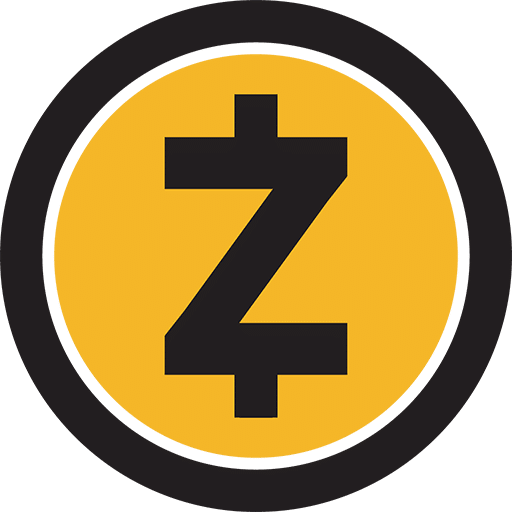
\includegraphics[width=1.5cm,height=1.5cm]{zcash}\\ \\
		\item{Kadena}\\ \\
		
\includegraphics[width=1.5cm,height=1.5cm]{kadena}\\ \\
	\end{itemize}
\end{itemize}


\section{Wie kann ich mit Kryptowährung Geld verdienen ?}
\subsection{Krypto-Mining}
\subsubsection{Konzept}
Im Jahr 2022 können wir die Preise der Währungen sehen, der Bitcoin liegt in diesem Monat bei 15.891 Euro, das ist ein astronomischer Preis für diese Währung. Also, wir sind daran interessiert, und wir wollen unsere Mining-Unternehmen zu starten. \\ \\ \\ 
Schauen wir uns an, was ein gutes Krypto-Mining-Rig ausmacht und welche Hardware man braucht, wenn man es mit dem Mining ernst meint. Und bevor wir direkt mit den notwendigen Materialien beginnen, möchte ich zuerst über ein sehr wichtiges Wort sprechen, das in dieser Branche verwendet wird. Was ist Krypto-Mining-Rig. \\ \\ \\ 
Also, Rig Computer enthält eine extrem leistungsstarke Materialien, die es eine Menge von Versorgungsmodulen enthält. Zum Beispiel: wenn jemand Bitcoin minen will, mit der riesigen Konkurrenz auf diese Kryptowährung, und die große Schwierigkeit. Ein normaler oder leistungsfähiger Computer wird für diese Aufgabe nicht ausreichen. Deshalb steht das Rig an erster Stelle, denn es enthält eine Hauptplatine, die eine oder mehrere Grafikkarten gleichzeitig bedienen kann. Wir verwenden GPU in dieser Operation, weil wir für die hohe mögliche Geschwindigkeit suchen, aber wenn es eine Menge von Grafikkarten, wird es auch notwendig sein, eine robuste Stromversorgung zu haben, um diese Operation auf das hohe Niveau zu schieben.
\newpage
\subsubsection{Hardware}
\begin{large}
	\textbf{Motherboard :} Asus B250 Mining Expert \\ \\
	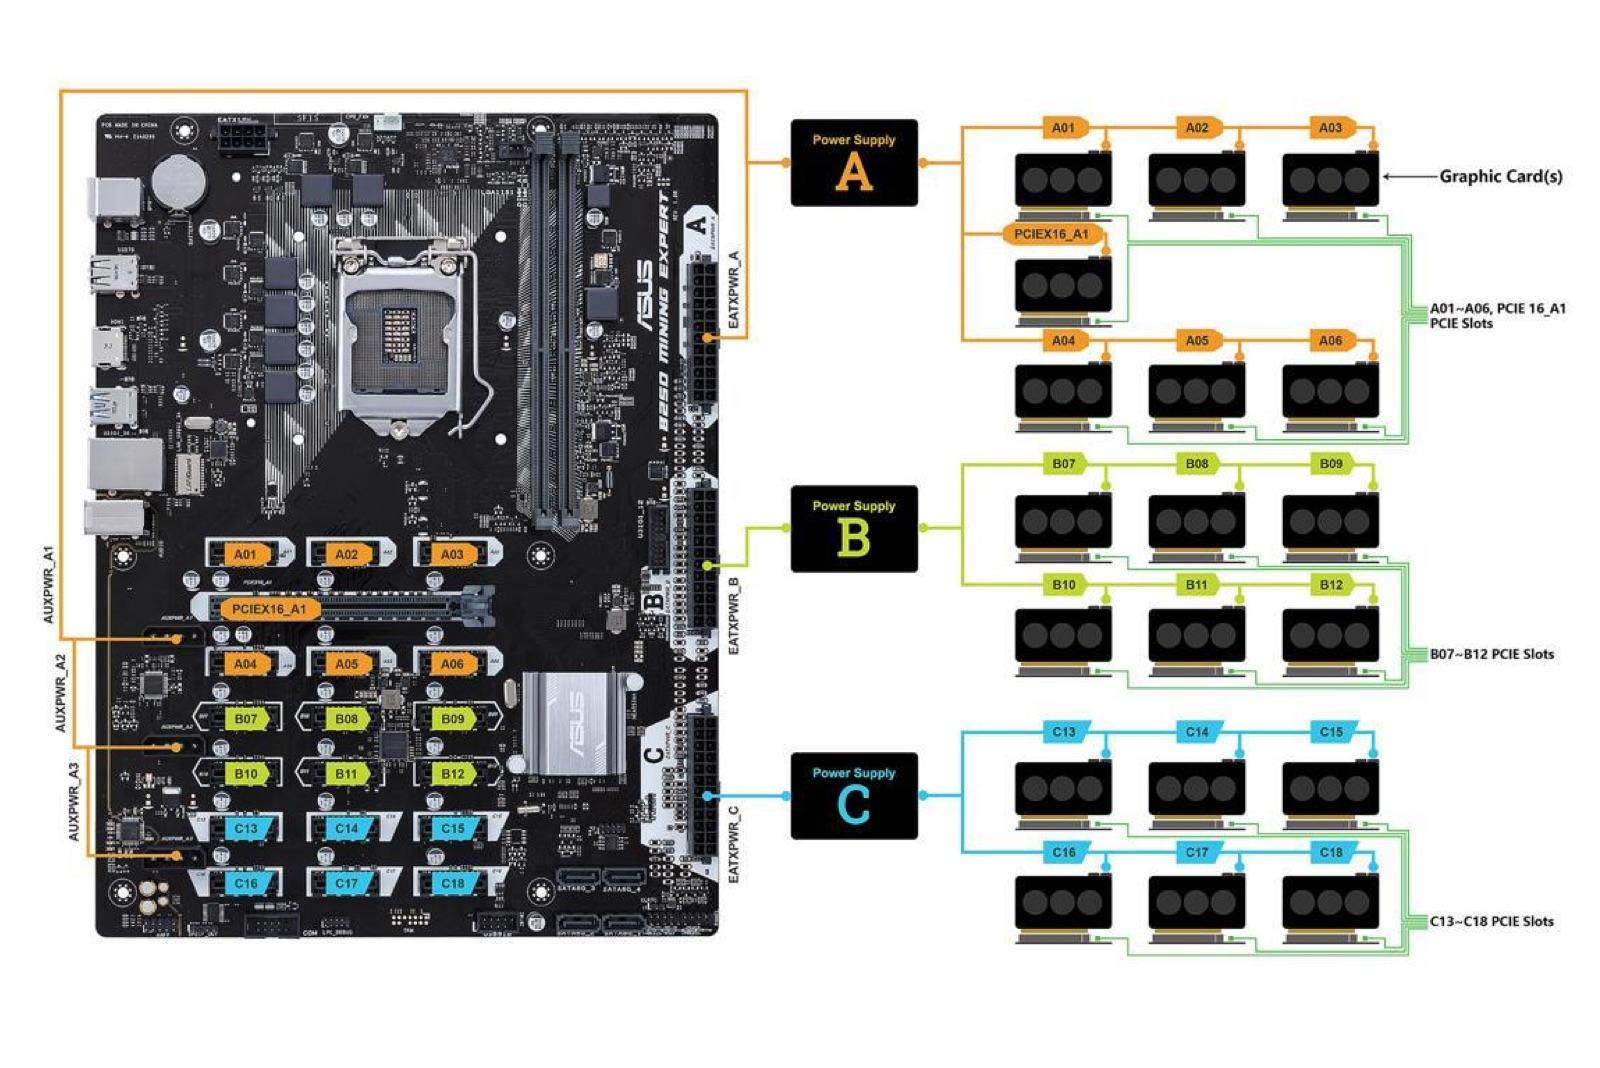
\includegraphics[width=15cm,height=15cm]{motherboard}  \\ \\
	Dieses Motherboard ist wirklich ein Biest, es wurde 2017 veröffentlicht und kann 19 angeschlossene Grafikkarten verarbeiten. Das ist wichtig für unser Setup.
	Das Unternehmen Asus hat empfohlene GPU-Layouts für 19 - 13 und 11 für dieses Board veröffentlicht. Es kann auch mit anderen Layouts umgehen, aber es wird empfohlen, sich an den Asus-Vorschlag zu halten.
	
\end{large}
\newpage
\begin{large}
	\textbf{CPU :} Intel Core i5-6500 \\ \\
	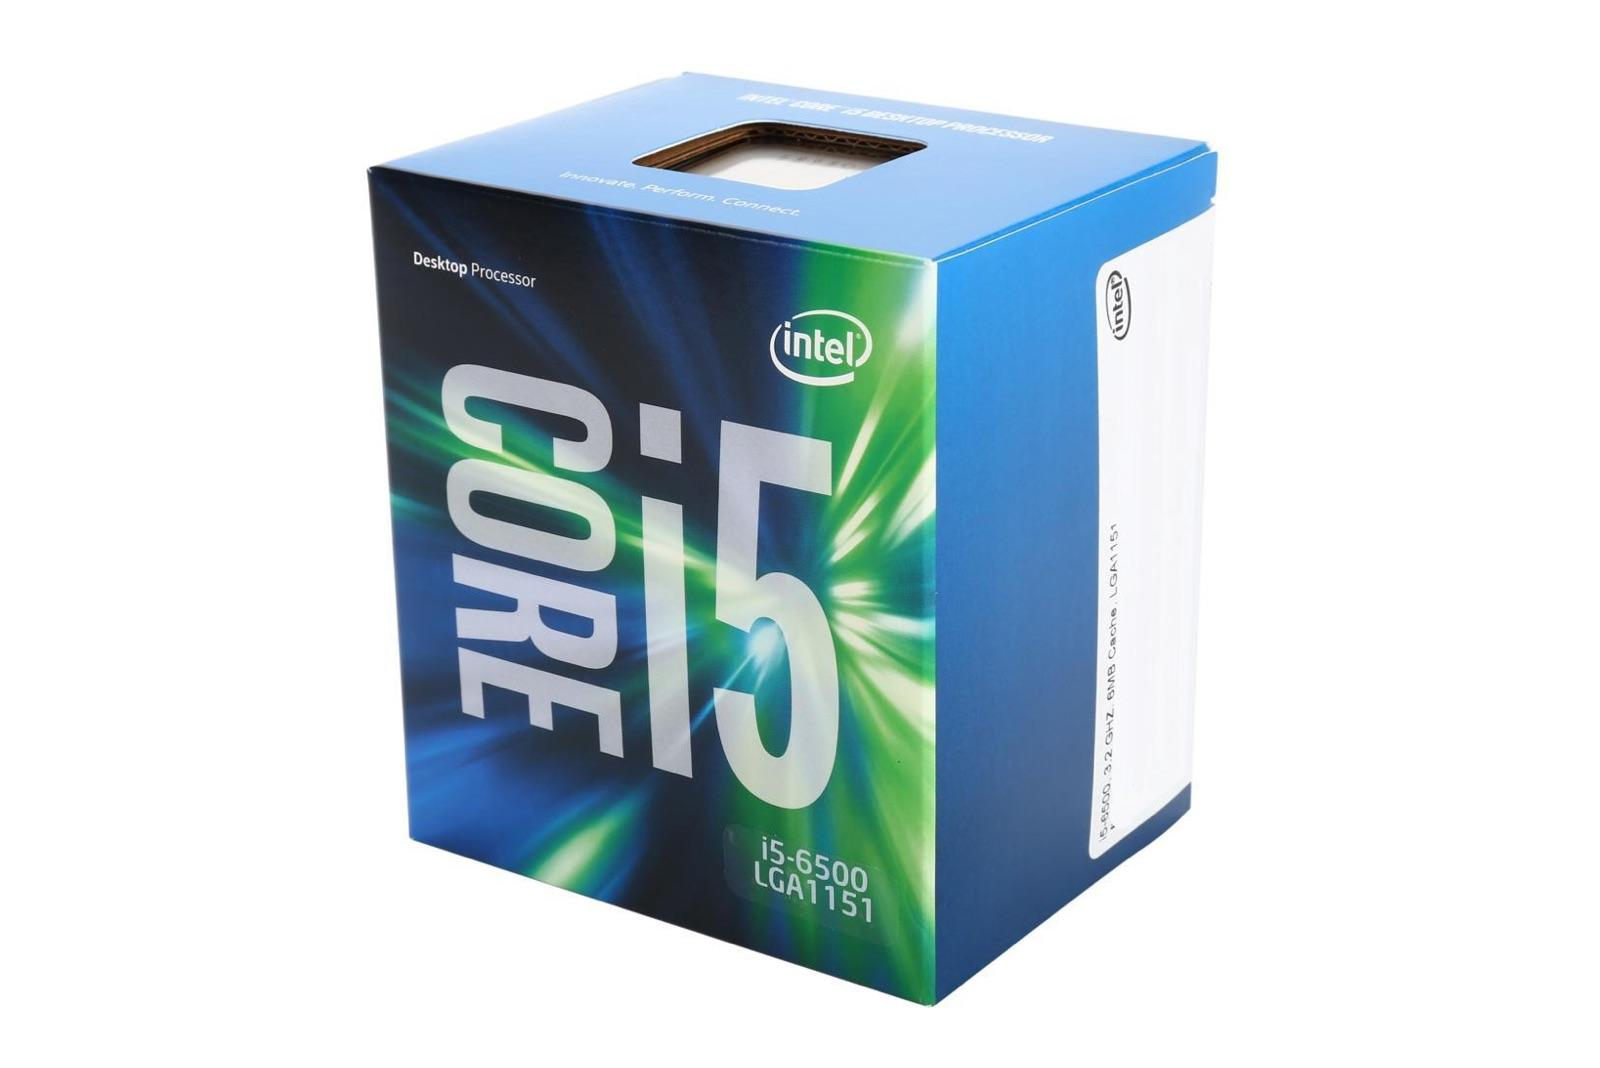
\includegraphics[width=10cm,height=8cm]{cpu}  \\ 
	Alle unsere massiven Operationen werden von der GPU ausgeführt, so dass wir kein Geld für eine leistungsstarke CPU ausgeben müssen, diese CPU hier eignet sich sehr gut für unser Setup und ist auch mit dem Motherboard kompatibel. \\ \\ \\
	
\end{large}
\begin{large}
	\textbf{RAM :} G.SKILL Aegis 16GB (2 x 8GB) \\ 
	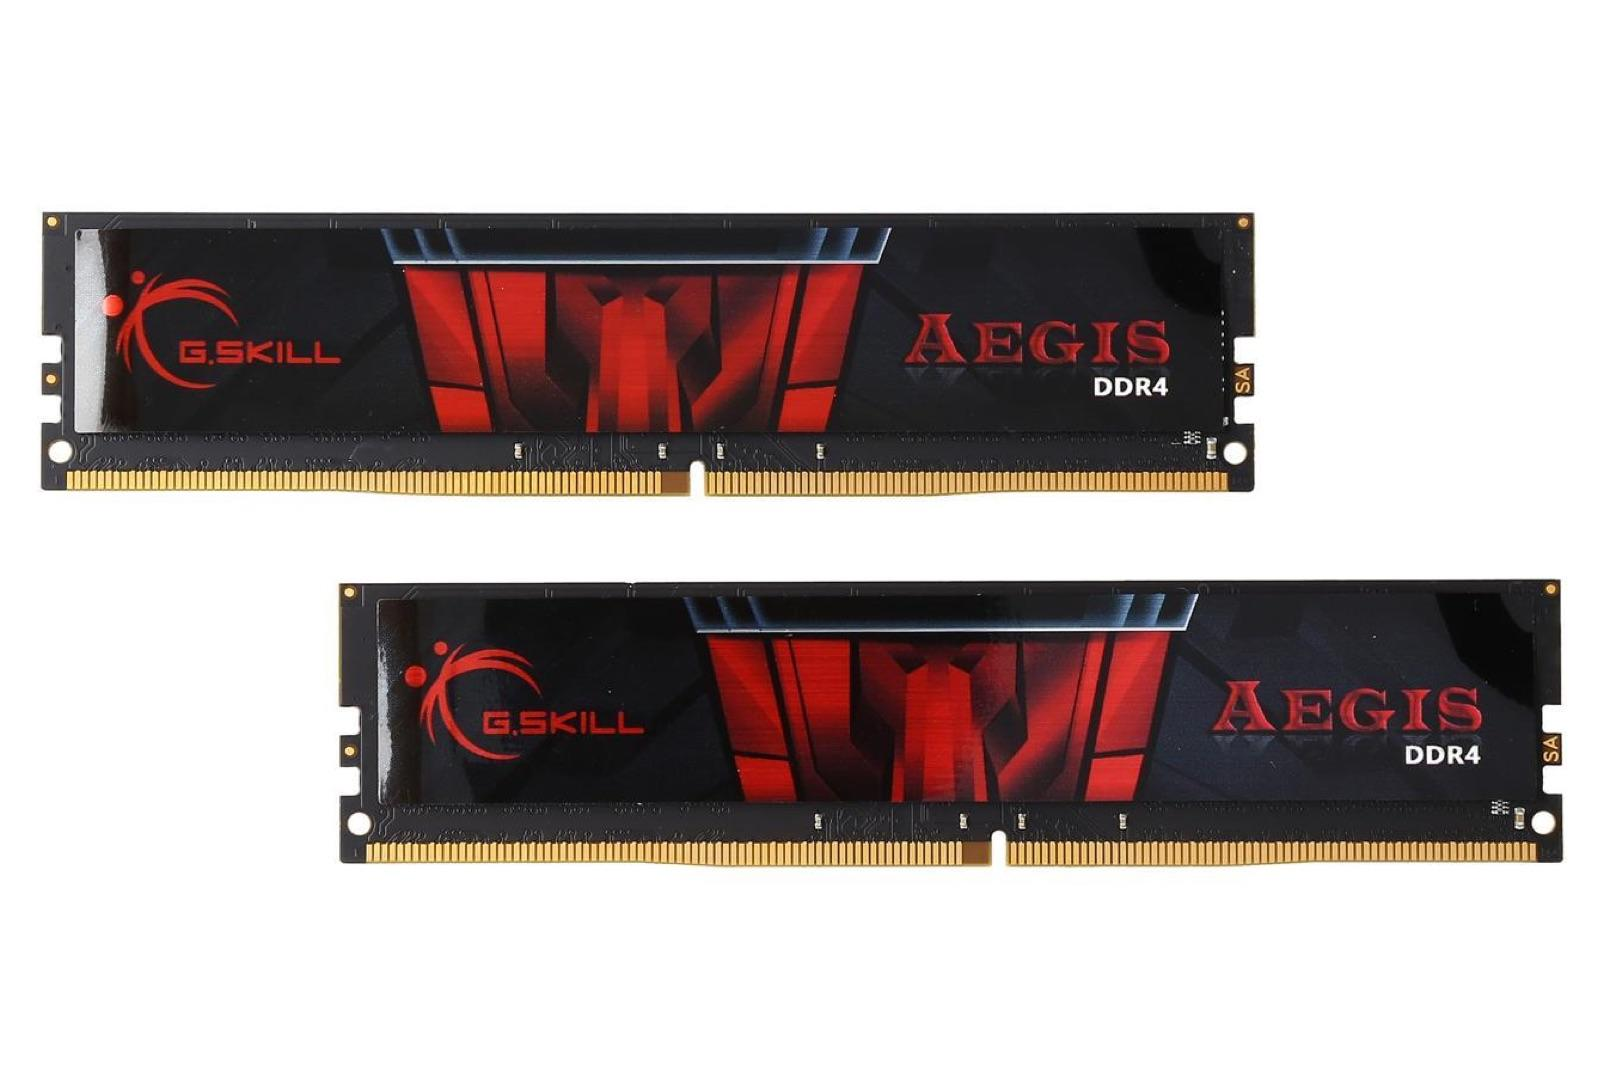
\includegraphics[width=\linewidth,height=5cm]{ram}  \\
	Es besteht auch keine Notwendigkeit, Geld für 128 GB RAM auszugeben, diese 16 GB (DDR4) reichen für unser Unternehmen aus und sind gut, um die Mission zu erfüllen. \\
	
	
	
\end{large}
\newpage
\begin{large}
	\textbf{Storage :} SanDisk SSD Plus 1TB \\ 
	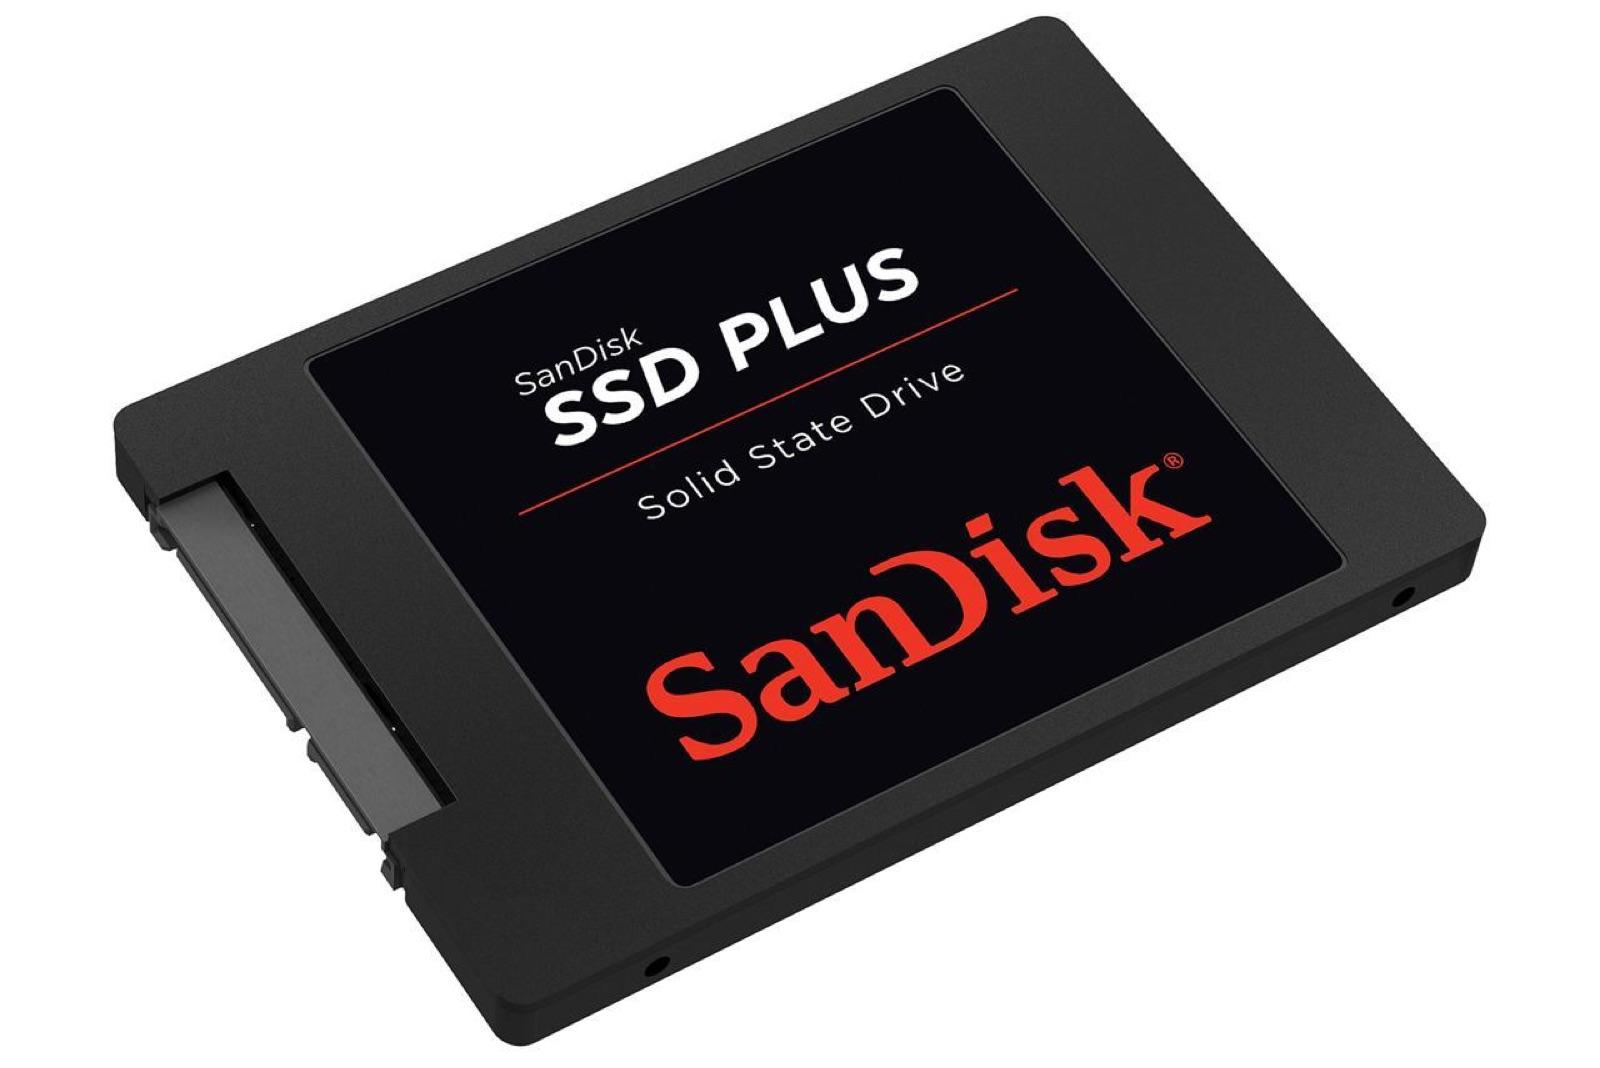
\includegraphics[width=\linewidth,height=5cm]{storage}  \\
	Ich werde es vorziehen, 4 seiner ssd-Speicher zu installieren. Sie sind schnell und unter 100\$	\\
\end{large}
\\ \\
\begin{large}
	\textbf{PSU :} Segotep 850W Full-Modular PSU \\ 
	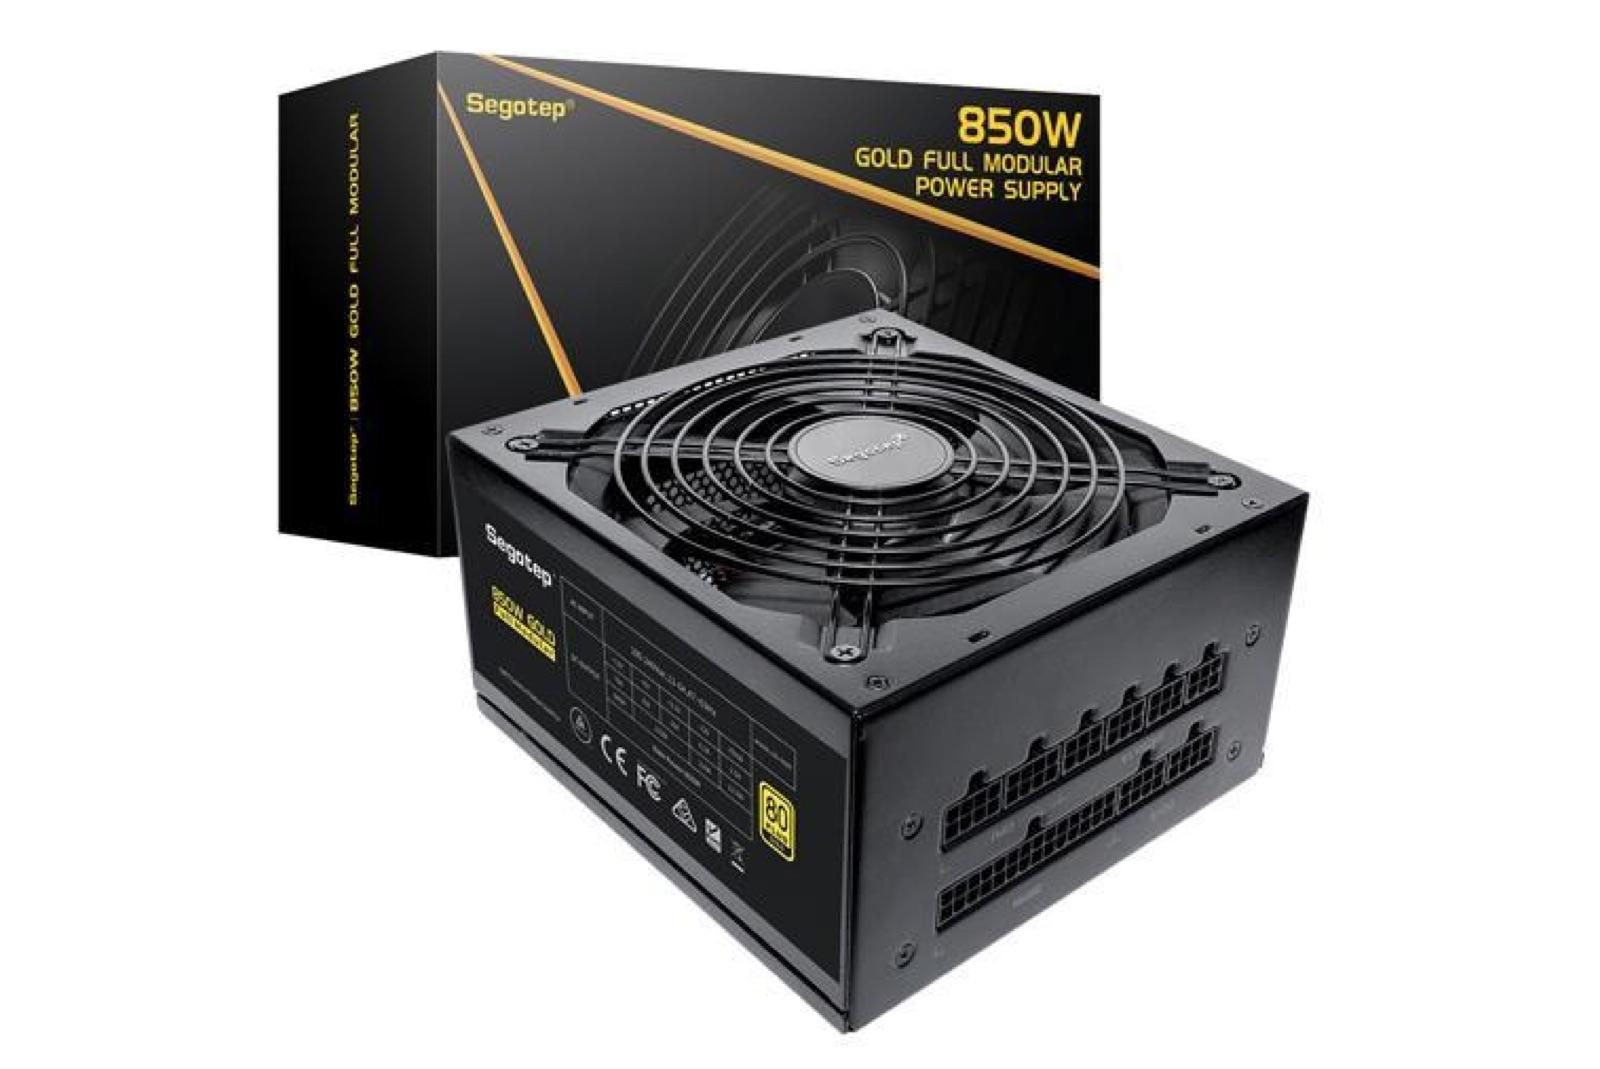
\includegraphics[width=\linewidth,height=5cm]{psu}  \\
	Diese "Segotep PSUs" sind gut, denn sie bieten eine zuverlässige Leistung, die davon abhängt, wie viele Grafikkarten Sie installiert haben, benötigen Sie möglicherweise mehrere PSUs. Aber wenn Sie Ihr Bitcoin-Mining auf extreme Leistung bringen wollen, ist es notwendig, mehr zu bezahlen \\
\end{large}
\newpage
\begin{large}
	\textbf{PCI-e Riser :} FebSmart 16x to 1x Powered Riser 6-pack \\ 
	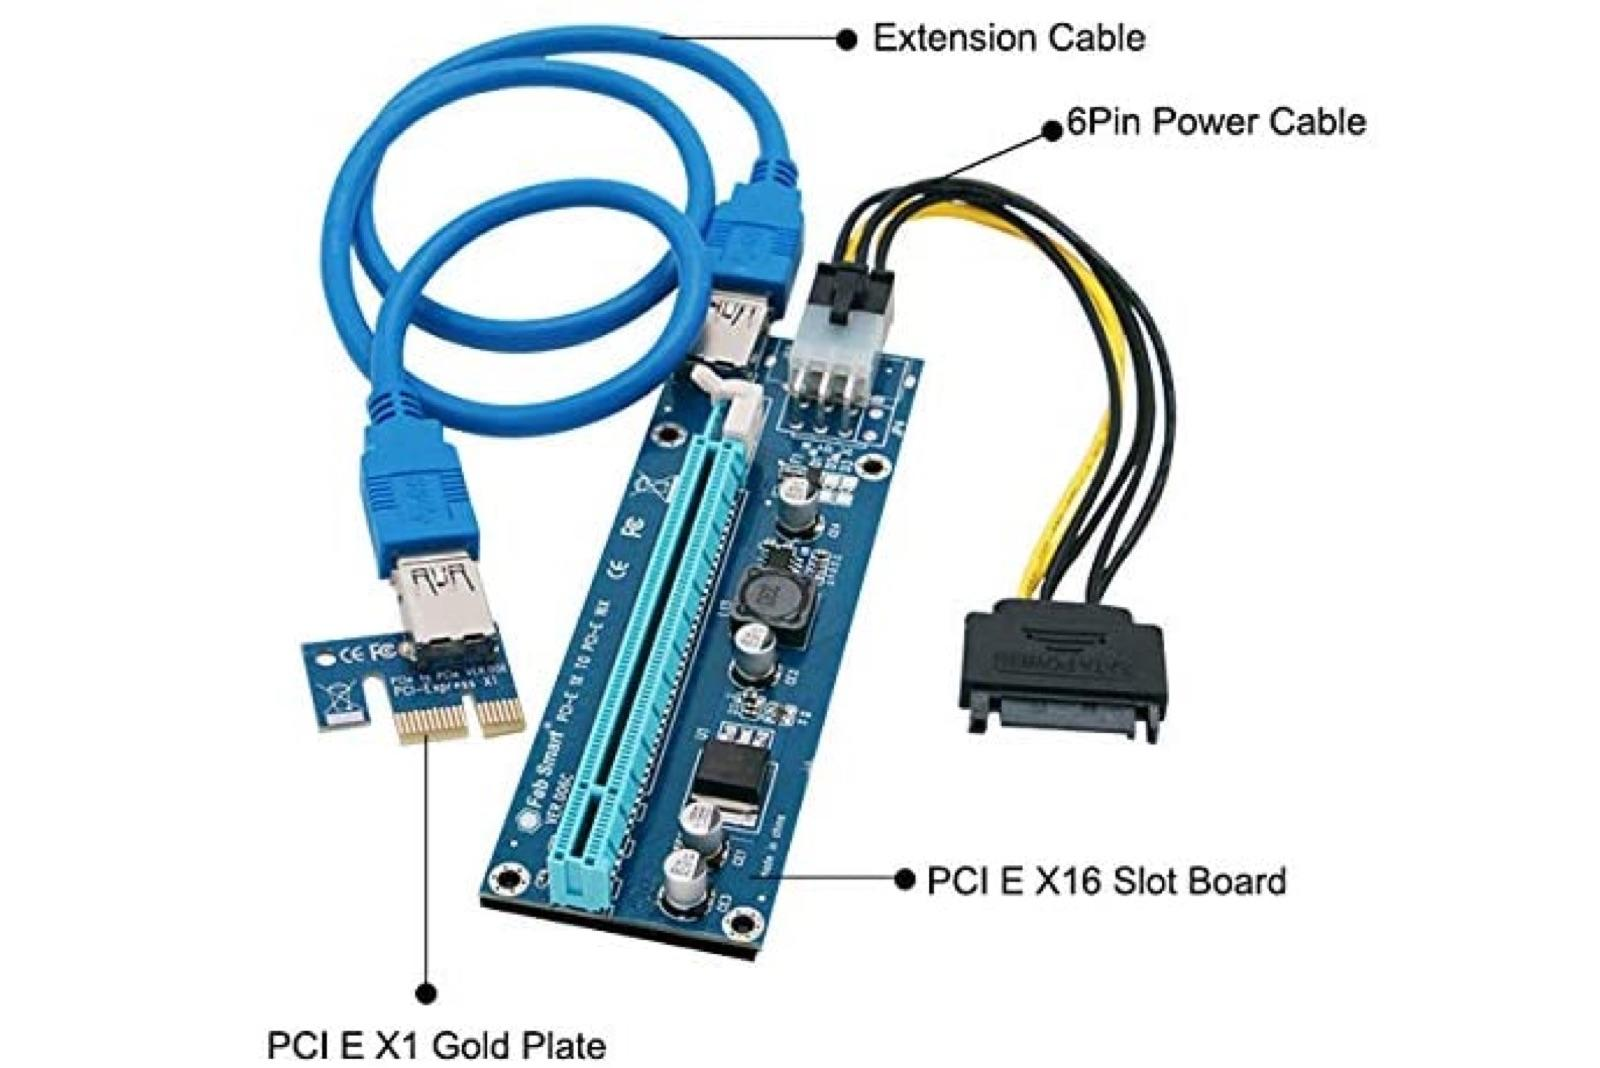
\includegraphics[width=\linewidth,height=5cm]{pci}  \\
	Dies ist der eigentliche Unterschied zwischen Rig und normalem Computer, denn man kann nicht alle Grafikkarten direkt an das Motherboard anschließen, aber mit diesem Modul kann man sie indirekt anschließen.\\ \\
	
	Ich empfehle die Verwendung von powered risers für jede Grafikkarte, da sie eine großartige und stabile Stromversorgung für die Grafikkarten bieten \\ \\ \\
	
	
\end{large}

\begin{large}
	\textbf{Nvidia graphics card :} MSI Ventus 3X GeForce RTX 3090
	 \\ 
	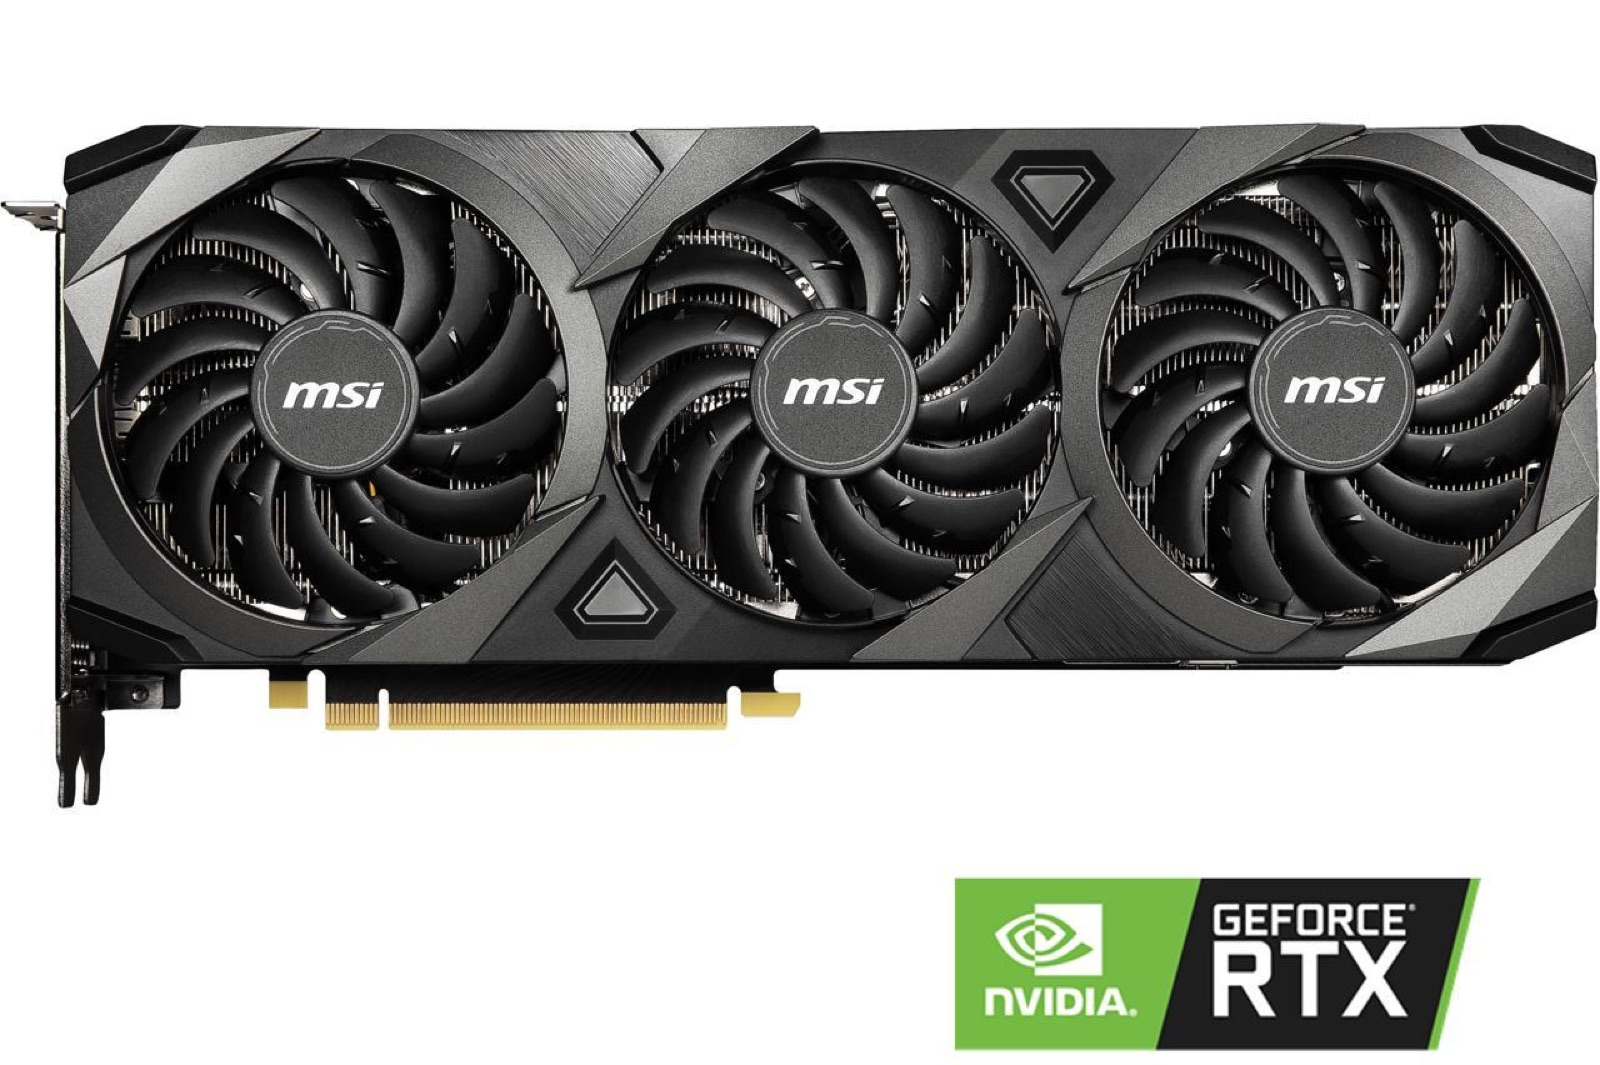
\includegraphics[width=\linewidth,height=5cm]{graphic}  \\
	Dies ist eine großartige Karte für ein Mining-Rig, fähig zur Übertaktung, stabil und gut gekühlt. Es ist eine ziemlich effiziente Karte, die niedrigeren Stromverbrauch und reduzierte Bergbaukosten bedeutet. \\ 

	
\end{large}
\newpage
\section{Wo sollte ich mein Geld in Kryptowährungen investieren?}
Diejenigen Investoren, die in den ersten Tagen in Bitcoin investiert haben, sind jetzt so reich und extrem wohlhabend geworden.
Der Blockchain-Markt wird immer größer und mächtiger, vor allem mit dem Web 3. Die Anleger suchen nach der nächsten digitalen Währung, um reich zu werden. Es wird nun die Frage gestellt, wie man die nächste große Kryptowährung finden kann.
\begin{itemize}
	\item Der Preis ist entscheidend\\
	Das wichtigste Element, auf das man bei der Suche nach Kryptowährungen achten sollte, ist der Preis des Tokens. Für die Investoren, die nicht über ein großes Budget verfügen, um in die Kryptowährungen zu investieren, sollten einige Kryptos mit einem niedrigen Preis kaufen.
	\item Aussichten auf Annahme\\
	Wenn jemand eine Kryptowährung finden kann, die einen Vorteil gegenüber anderen hat (und die mehr angenommen wird). Es wird die beste Kryptowährung sein, in die Sie Ihr Geld investieren sollten.
	\item Die Versorgung ist ein Faktor\\
	Die meisten Kryptowährungen haben ein vorher festgelegtes maximales Angebot. Wenn das Maximum durch die Mining-Operationen erreicht wird. Wenn das Interesse aufrechterhalten wird, während das Angebot festgelegt ist, könnte der Preis steigen. Behalten Sie also immer im Hinterkopf, dass das Angebot ein wichtiger Faktor ist, bevor Sie investieren
	\item Preis und Volumen
	Im Jahr 2022 gibt es viele Plattformen, die das Investieren so einfach machen, es speichert die wechselnde Geschichte der Kryptowährungen und die Preise über den Blockchain-Markt. Es ist also besser, den Markt sehr sorgfältig zu scannen und eine Entscheidung über die Erhöhung der Währungen zu treffen. Es gibt auch einige künstliche intelligente Modelle, die auf alten Kryptowährungsdaten basieren und die es leicht machen, vorherzusagen, ob der Preis einer Kryptowährung in Zukunft steigen oder fallen wird.
	Aber Sie sollten bedenken, dass der Preis nicht gehalten werden kann, und es gibt immer eine Chance zu verlieren. 
\end{itemize}

%\subsection{Wie kann ich mein geld anlegen ?}
\chapter{Schluss}
Die Methode \textquestiondown Proof-Of-Work\textquotedblright ist ein Konsensmechanismus, der es den Netzwerkteilnehmern ermöglicht zu bestätigen, dass die von ihnen durchgeführten Transaktionen gültig sind. Dies geschieht, indem andere Miner versuchen, eine gültige Nonce zu finden. Der erste, der die Nonce findet, erhält eine Belohnung, und die anderen Teilnehmer überprüfen die Gültigkeit des Hashs. Das Mining erfordert eine starke Hardware-Ausstattung, aber alles wird mietbar sein.\\ \\ \\

Nach diesem Bericht haben wir viele Informationen über bitcoin und seine Funktionsweise und die grundlegende Funktion des Proof of Work gesehen. Wir verstehen auch die Bedeutung des Blockchain-Netzwerks und alle anderen Definitionen. Lassen Sie uns beginnen, in Bitcoin oder in andere Kryptowährungen zu investieren.\\

\newpage
\begin{center}
	\begin{LARGE}
		\textbf{Literatur}
	\end{LARGE}
\end{center}

\url{https://de.wikipedia.org/wiki/Blockchain} \\ \\
\url{https://www.softwaretestinghelp.com/wp-content/qa/uploads/2019/06/structure-of-a-singly-linked-list.png} \\ \\
\url{https://en.wikipedia.org/wiki/Proof\_of\_work} \\ \\
\url{https://en.wikipedia.org/wiki/Blockchain} \\ \\
\url{https://www.iotforall.com/blockchain-use-cases-in-2022} \\ \\

\url{https://www.btc-echo.de/academy/bibliothek/proof-of-work/} \\ \\
\url{https://www.fool.com/investing/stock-market/market-sectors/financials/cryptocurrency-stocks/proof-of-work/} \\ \\
\url{https://www.blockchain.com/explorer/api/blockchain\_api}\\ \\
\url{https://bitcoin.org/img/icons/opengraph.png}\\ \\


\url{https://upload.wikimedia.org/wikipedia/commons/5/58/Bitcoin_Cash.png} \\ \\
\url{https://upload.wikimedia.org/wikipedia/commons/c/c1/Bsv-icon-small.png} \\ \\
\url{https://s2.coinmarketcap.com/static/img/coins/200x200/2083.png} \\ \\ 
\url{https://www.creativefabrica.com/wp-content/uploads/2021/06/16/Cryptocurrency-Litecoin-Logo-Graphics-13458855-1.jpg} \\ \\
\url{https://block-builders.de/wp-content/uploads/2021/01/ony3qesa3ebx-1024x1024.png} \\ \\
\url{https://s2.coinmarketcap.com/static/img/coins/200x200/1321.png} \\ \\
\url{https://s2.coinmarketcap.com/static/img/coins/200x200/328.png}\\ \\ 
\url{https://z.cash/wp-content/uploads/2018/10/zcash-logo-fullcolor-512sq.png}\\ \\
\url{https://s2.coinmarketcap.com/static/img/coins/200x200/5647.png} \\ \\
\url{https://s2.coinmarketcap.com/static/img/coins/200x200/2577.png} \\ \\
\url{https://s2.coinmarketcap.com/static/img/coins/200x200/1042.png} \\ \\
\url{https://s2.coinmarketcap.com/static/img/coins/64x64/1698.png} \\ \\
\url{https://s2.coinmarketcap.com/static/img/coins/200x200/109.png} \\ \\


\url{https://www.fool.com/investing/stock-market/market-sectors/financials/cryptocurrency-stocks/proof-of-work/#:~:text=The%20proof%2Dof%2Dwork%20algorithm,too%20slowly%2C%20they%20get%20easier.} \\ \\
\url{https://www.blockchain.com/explorer/api/blockchain_api} \\ \\
\url{https://bitcoin.org/img/icons/opengraph.png?1666775325} \\ \\
\url{https://block-builders.de/wp-content/uploads/2021/01/ony3qesa3ebx-1024x1024.png} \\ \\
\url{https://www.creativefabrica.com/wp-content/uploads/2021/06/16/Cryptocurrency-Litecoin-Logo-Graphics-13458855-1.jpg}\\
\url{https://www.creativefabrica.com/wp-content/uploads/2021/06/16/Cryptocurrency-Litecoin-Logo-Graphics-13458855-1.jpg}\\ \\
\url{https://www.investopedia.com/terms/p/proof-stake-pos.asp#:~:text=What%20Is%20Proof%2Dof%2DStake%20vs.,new%20blocks%20to%20the%20blockchain.}\\ \\
\url{https://www.businessinsider.com/personal-finance/proof-of-work}\\ \\
\url{https://smartasset.com/investing/how-to-invest-in-cryptocurrency#:~:text=The%20most%20popular%20place%20to,Ethereum%20with%20a%20debit%20card.}\\ \\
\url{https://www.zdnet.com/article/how-to-build-a-cryptomining-rig/}\\ \\
\url{https://www.investopedia.com/news/how-identify-next-big-cryptocurrency/}\\ \\

\end{document}
